\documentclass[10pt,journal,compsoc]{IEEEtran}

% Some very useful LaTeX packages include:
% (uncomment the ones you want to load)


% *** MISC UTILITY PACKAGES ***
%
%\usepackage{ifpdf}
% Heiko Oberdiek's ifpdf.sty is very useful if you need conditional
% compilation based on whether the output is pdf or dvi.
% usage:
% \ifpdf
%   % pdf code
% \else
%   % dvi code
% \fi
% The latest version of ifpdf.sty can be obtained from:
% http://www.ctan.org/tex-archive/macros/latex/contrib/oberdiek/
% Also, note that IEEEtran.cls V1.7 and later provides a builtin
% \ifCLASSINFOpdf conditional that works the same way.
% When switching from latex to pdflatex and vice-versa, the compiler may
% have to be run twice to clear warning/error messages.






% *** CITATION PACKAGES ***
%
\ifCLASSOPTIONcompsoc
  % IEEE Computer Society needs nocompress option
  % requires cite.sty v4.0 or later (November 2003)
  \usepackage[nocompress]{cite}
\else
  % normal IEEE
  \usepackage{cite}
\fi
% cite.sty was written by Donald Arseneau
% V1.6 and later of IEEEtran pre-defines the format of the cite.sty package
% \cite{} output to follow that of IEEE. Loading the cite package will
% result in citation numbers being automatically sorted and properly
% "compressed/ranged". e.g., [1], [9], [2], [7], [5], [6] without using
% cite.sty will become [1], [2], [5]--[7], [9] using cite.sty. cite.sty's
% \cite will automatically add leading space, if needed. Use cite.sty's
% noadjust option (cite.sty V3.8 and later) if you want to turn this off
% such as if a citation ever needs to be enclosed in parenthesis.
% cite.sty is already installed on most LaTeX systems. Be sure and use
% version 5.0 (2009-03-20) and later if using hyperref.sty.
% The latest version can be obtained at:
% http://www.ctan.org/tex-archive/macros/latex/contrib/cite/
% The documentation is contained in the cite.sty file itself.
%
% Note that some packages require special options to format as the Computer
% Society requires. In particular, Computer Society  papers do not use
% compressed citation ranges as is done in typical IEEE papers
% (e.g., [1]-[4]). Instead, they list every citation separately in order
% (e.g., [1], [2], [3], [4]). To get the latter we need to load the cite
% package with the nocompress option which is supported by cite.sty v4.0
% and later. Note also the use of a CLASSOPTION conditional provided by
% IEEEtran.cls V1.7 and later.





% *** GRAPHICS RELATED PACKAGES ***
%
\ifCLASSINFOpdf
    \usepackage[pdftex]{graphicx}
  % declare the path(s) where your graphic files are
    \graphicspath{{./pics/}}
  % and their extensions so you won't have to specify these with
  % every instance of \includegraphics
  %  \DeclareGraphicsExtensions{.pdf,.jpeg,.png}
\else
  % or other class option (dvipsone, dvipdf, if not using dvips). graphicx
  % will default to the driver specified in the system graphics.cfg if no
  % driver is specified.
  % \usepackage[dvips]{graphicx}
  % declare the path(s) where your graphic files are
  % \graphicspath{{../eps/}}
  % and their extensions so you won't have to specify these with
  % every instance of \includegraphics
  % \DeclareGraphicsExtensions{.eps}
\fi
% graphicx was written by David Carlisle and Sebastian Rahtz. It is
% required if you want graphics, photos, etc. graphicx.sty is already
% installed on most LaTeX systems. The latest version and documentation
% can be obtained at:
% http://www.ctan.org/tex-archive/macros/latex/required/graphics/
% Another good source of documentation is "Using Imported Graphics in
% LaTeX2e" by Keith Reckdahl which can be found at:
% http://www.ctan.org/tex-archive/info/epslatex/
%
% latex, and pdflatex in dvi mode, support graphics in encapsulated
% postscript (.eps) format. pdflatex in pdf mode supports graphics
% in .pdf, .jpeg, .png and .mps (metapost) formats. Users should ensure
% that all non-photo figures use a vector format (.eps, .pdf, .mps) and
% not a bitmapped formats (.jpeg, .png). IEEE frowns on bitmapped formats
% which can result in "jaggedy"/blurry rendering of lines and letters as
% well as large increases in file sizes.
%
% You can find documentation about the pdfTeX application at:
% http://www.tug.org/applications/pdftex






% *** MATH PACKAGES ***
%
\usepackage[cmex10]{amsmath}
% A popular package from the American Mathematical Society that provides
% many useful and powerful commands for dealing with mathematics. If using
% it, be sure to load this package with the cmex10 option to ensure that
% only type 1 fonts will utilized at all point sizes. Without this option,
% it is possible that some math symbols, particularly those within
% footnotes, will be rendered in bitmap form which will result in a
% document that can not be IEEE Xplore compliant!
%
% Also, note that the amsmath package sets \interdisplaylinepenalty to 10000
% thus preventing page breaks from occurring within multiline equations. Use:
\interdisplaylinepenalty=2500
% after loading amsmath to restore such page breaks as IEEEtran.cls normally
% does. amsmath.sty is already installed on most LaTeX systems. The latest
% version and documentation can be obtained at:
% http://www.ctan.org/tex-archive/macros/latex/required/amslatex/math/





% *** SPECIALIZED LIST PACKAGES ***
%
%\usepackage{algorithmic}
% algorithmic.sty was written by Peter Williams and Rogerio Brito.
% This package provides an algorithmic environment fo describing algorithms.
% You can use the algorithmic environment in-text or within a figure
% environment to provide for a floating algorithm. Do NOT use the algorithm
% floating environment provided by algorithm.sty (by the same authors) or
% algorithm2e.sty (by Christophe Fiorio) as IEEE does not use dedicated
% algorithm float types and packages that provide these will not provide
% correct IEEE style captions. The latest version and documentation of
% algorithmic.sty can be obtained at:
% http://www.ctan.org/tex-archive/macros/latex/contrib/algorithms/
% There is also a support site at:
% http://algorithms.berlios.de/index.html
% Also of interest may be the (relatively newer and more customizable)
% algorithmicx.sty package by Szasz Janos:
% http://www.ctan.org/tex-archive/macros/latex/contrib/algorithmicx/




% *** ALIGNMENT PACKAGES ***
%
\usepackage{array}
% Frank Mittelbach's and David Carlisle's array.sty patches and improves
% the standard LaTeX2e array and tabular environments to provide better
% appearance and additional user controls. As the default LaTeX2e table
% generation code is lacking to the point of almost being broken with
% respect to the quality of the end results, all users are strongly
% advised to use an enhanced (at the very least that provided by array.sty)
% set of table tools. array.sty is already installed on most systems. The
% latest version and documentation can be obtained at:
% http://www.ctan.org/tex-archive/macros/latex/required/tools/


% IEEEtran contains the IEEEeqnarray family of commands that can be used to
% generate multiline equations as well as matrices, tables, etc., of high
% quality.




% *** SUBFIGURE PACKAGES ***
\ifCLASSOPTIONcompsoc
  \usepackage[caption=false,font=footnotesize,labelfont=sf,textfont=sf]{subfig}
\else
  \usepackage[caption=false,font=footnotesize]{subfig}
\fi
% subfig.sty, written by Steven Douglas Cochran, is the modern replacement
% for subfigure.sty, the latter of which is no longer maintained and is
% incompatible with some LaTeX packages including fixltx2e. However,
% subfig.sty requires and automatically loads Axel Sommerfeldt's caption.sty
% which will override IEEEtran.cls' handling of captions and this will result
% in non-IEEE style figure/table captions. To prevent this problem, be sure
% and invoke subfig.sty's "caption=false" package option (available since
% subfig.sty version 1.3, 2005/06/28) as this is will preserve IEEEtran.cls
% handling of captions.
% Note that the Computer Society format requires a sans serif font rather
% than the serif font used in traditional IEEE formatting and thus the need
% to invoke different subfig.sty package options depending on whether
% compsoc mode has been enabled.
%
% The latest version and documentation of subfig.sty can be obtained at:
% http://www.ctan.org/tex-archive/macros/latex/contrib/subfig/




% *** FLOAT PACKAGES ***
%
\usepackage{fixltx2e}
% fixltx2e, the successor to the earlier fix2col.sty, was written by
% Frank Mittelbach and David Carlisle. This package corrects a few problems
% in the LaTeX2e kernel, the most notable of which is that in current
% LaTeX2e releases, the ordering of single and double column floats is not
% guaranteed to be preserved. Thus, an unpatched LaTeX2e can allow a
% single column figure to be placed prior to an earlier double column
% figure. The latest version and documentation can be found at:
% http://www.ctan.org/tex-archive/macros/latex/base/


%\usepackage{stfloats}
% stfloats.sty was written by Sigitas Tolusis. This package gives LaTeX2e
% the ability to do double column floats at the bottom of the page as well
% as the top. (e.g., "\begin{figure*}[!b]" is not normally possible in
% LaTeX2e). It also provides a command:
%\fnbelowfloat
% to enable the placement of footnotes below bottom floats (the standard
% LaTeX2e kernel puts them above bottom floats). This is an invasive package
% which rewrites many portions of the LaTeX2e float routines. It may not work
% with other packages that modify the LaTeX2e float routines. The latest
% version and documentation can be obtained at:
% http://www.ctan.org/tex-archive/macros/latex/contrib/sttools/
% Do not use the stfloats baselinefloat ability as IEEE does not allow
% \baselineskip to stretch. Authors submitting work to the IEEE should note
% that IEEE rarely uses double column equations and that authors should try
% to avoid such use. Do not be tempted to use the cuted.sty or midfloat.sty
% packages (also by Sigitas Tolusis) as IEEE does not format its papers in
% such ways.
% Do not attempt to use stfloats with fixltx2e as they are incompatible.
% Instead, use Morten Hogholm'a dblfloatfix which combines the features
% of both fixltx2e and stfloats:
%
% \usepackage{dblfloatfix}
% The latest version can be found at:
% http://www.ctan.org/tex-archive/macros/latex/contrib/dblfloatfix/




%\ifCLASSOPTIONcaptionsoff
%  \usepackage[nomarkers]{endfloat}
% \let\MYoriglatexcaption\caption
% \renewcommand{\caption}[2][\relax]{\MYoriglatexcaption[#2]{#2}}
%\fi
% endfloat.sty was written by James Darrell McCauley, Jeff Goldberg and
% Axel Sommerfeldt. This package may be useful when used in conjunction with
% IEEEtran.cls'  captionsoff option. Some IEEE journals/societies require that
% submissions have lists of figures/tables at the end of the paper and that
% figures/tables without any captions are placed on a page by themselves at
% the end of the document. If needed, the draftcls IEEEtran class option or
% \CLASSINPUTbaselinestretch interface can be used to increase the line
% spacing as well. Be sure and use the nomarkers option of endfloat to
% prevent endfloat from "marking" where the figures would have been placed
% in the text. The two hack lines of code above are a slight modification of
% that suggested by in the endfloat docs (section 8.4.1) to ensure that
% the full captions always appear in the list of figures/tables - even if
% the user used the short optional argument of \caption[]{}.
% IEEE papers do not typically make use of \caption[]'s optional argument,
% so this should not be an issue. A similar trick can be used to disable
% captions of packages such as subfig.sty that lack options to turn off
% the subcaptions:
% For subfig.sty:
% \let\MYorigsubfloat\subfloat
% \renewcommand{\subfloat}[2][\relax]{\MYorigsubfloat[]{#2}}
% However, the above trick will not work if both optional arguments of
% the \subfloat command are used. Furthermore, there needs to be a
% description of each subfigure *somewhere* and endfloat does not add
% subfigure captions to its list of figures. Thus, the best approach is to
% avoid the use of subfigure captions (many IEEE journals avoid them anyway)
% and instead reference/explain all the subfigures within the main caption.
% The latest version of endfloat.sty and its documentation can obtained at:
% http://www.ctan.org/tex-archive/macros/latex/contrib/endfloat/
%
% The IEEEtran \ifCLASSOPTIONcaptionsoff conditional can also be used
% later in the document, say, to conditionally put the References on a
% page by themselves.




% *** PDF, URL AND HYPERLINK PACKAGES ***
%
%\usepackage{url}
% url.sty was written by Donald Arseneau. It provides better support for
% handling and breaking URLs. url.sty is already installed on most LaTeX
% systems. The latest version and documentation can be obtained at:
% http://www.ctan.org/tex-archive/macros/latex/contrib/url/
% Basically, \url{my_url_here}.





% *** Do not adjust lengths that control margins, column widths, etc. ***
% *** Do not use packages that alter fonts (such as pslatex).         ***
% There should be no need to do such things with IEEEtran.cls V1.6 and later.
% (Unless specifically asked to do so by the journal or conference you plan
% to submit to, of course. )

\usepackage{enumitem}
%\usepackage[]{algorithm2e}
\usepackage[]{algpseudocode}
\usepackage{algorithm}
\usepackage{multirow}
\usepackage{slashbox}
\usepackage{color}
%\usepackage{ulem}
%\usepackage[numbers,sort&compress]{natbib}
\renewcommand{\arraystretch}{1.3}


\usepackage{color}

% correct bad hyphenation here
\hyphenation{op-tical net-works semi-conduc-tor}

\newcommand{\tabincell}[2]{\begin{tabular}{@{}#1@{}}#2\end{tabular}}

\floatname{algorithm}{Algorithm}

\begin{document}
\title{Efficient, Robust and Exact Boolean Operations on N Triangular Mesh Primitives}
\author{Rui~Wang,~
        Xudong~Jiang,~
        Hongbo~Fu,~
        Bin~Sheng,~and
        Enhua~Wu
\IEEEcompsocitemizethanks{

\IEEEcompsocthanksitem R. Wang and B. Sheng are with the Department of Computer Science and Engineering, Shanghai Jiao Tong University. Email:\{jhcz,shengbin\}@sjtu.edu.cn

\IEEEcompsocthanksitem X. Jiang is with Autodesk China Research \& Development Center. Email: xudong.jiang@autodesk.com

\IEEEcompsocthanksitem H. Fu is with the School of Creative Media, City University of Hong Kong. Email: hongbofu@cityu.edu.hk


\IEEEcompsocthanksitem E. Wu is currently a research professor at State Key Lab. of Computer Science, Institute of Software, Chinese Academy of Sciences. Email: ehwu@umac.mo}
}

%\markboth{Journal of \LaTeX\ Class Files,~Vol.~13, No.~9, September~2014}%
%{Shell \MakeLowercase{\textit{et al.}}: Bare Demo of IEEEtran.cls for Computer Society Journals}

\IEEEtitleabstractindextext{
\begin{abstract}
  In this paper, we propose an efficient non-incremental approach to evaluate the boundary of constructive solid geometry (CSG). The face membership classification step is a bottleneck in many existing CSG evaluation approaches. The key idea of our approach is to use local coherence of space labels to accelerate this step. We employ a two-level grouping scheme to group faces that share the same space labels. Therefore, these common space labels can be shared within each group to avoid repetitive computation. Our method is optimized for a non-incremental evaluation. It generates the entire result model at once, rather than performing a step-by-step evaluation of Boolean operations. To achieve a robust evaluation, our approach introduces plane-based geometry into the intersection computation step. Comparison experiments with state-of-the-art techniques show that our method can more efficiently perform boundary evaluation of both trivial and complicated CSG with massive faces while maintaining robustness.
\end{abstract}


\begin{IEEEkeywords}
Boolean operations, triangle mesh, CSG evaluation, plane-based geometry.
\end{IEEEkeywords}

}



\maketitle


\IEEEdisplaynontitleabstractindextext
\IEEEpeerreviewmaketitle

\IEEEraisesectionheading{\section{Introduction}\label{sec:introduction}}
\IEEEPARstart{C}{onstructive} solid geometry (CSG) has long been a popular modeling tool of computer-aided design and computer-aided manufacturing (CAD/CAM). It constructs complex models by combining primitives using a series of regularized Boolean operations \cite{requicha1977mathematical}: union, intersection and difference. CSG is often represented by a binary tree, called a CSG tree, whose leaves are primitives and whose internal nodes are Boolean operations.

CSG can be converted into the widely-used  boundary representation (i.e., triangle mesh) through boundary evaluation. It is an classical topic with history of over three decades. However, one always have to make a bargain between robustness and efficiency of the boundary evaluation. One could use rational number arithmetic to avoid errors and thus ensure unconditional robustness, which could be over 20 times slower than a non-robust one [?]. On the other hand, using an approximate method for boundary evaluation can be very fast, but lack exactness.

Most recent methods [???] try to find a faster way to evaluate boundary of CSG, yet for robustness, the answers are often ambiguous workarounds, like setting a tolerance [?], using higher precision float point number [?] or rotating the primitive with small angle to avoid coplanar cases [?], etc. These tricks are often too vague to implement, heavily depend on the experiments, thus not reliable. Campen et. al. [?] gave a good paradigm of a unconditional robust and exact boundary evaluation methods. It proved to be fairly efficient, and never crashed with legal inputs. Since then, few exact evaluation methods declare themselves as an unconditional robust one.

We prove that exact boundary evaluation of CSG can be even faster, while keeping unconditional robust. We adapt the plane-based techniques of Campen et. al.'s method for robustness, but use a framework very different from Campen et. al.'s, taking advantage of the recent popular idea of using geometry connectivity for face classification acceleration. In addition, unlike many other methods, our method can perform boundary evaluation directly for CSG with more than two primitives. That is, we do not incrementally generate the intermediate meshes of each Boolean operation. In opposite, we generate the final mesh directly. In this way, extra complexity of method is introduced, but we can save much computation time. The experiment shows that our method is much faster than Campen et. al.'s method, while only about twice slower than the state-of-art non-robust methods [??].



\section{Related Work}

\subsection{Plane-based geometry representation}

The primary information of commonly used representation of solids are the vertex coordinates. In this way, edges and faces are implicitly represented by combination of vertices. In contrast, in plane-based representation, the primary elements are planes. Vertices and edges are all implicitly represented by plane intersections.



The concept of plane-based representation of polygonal meshes was first described by Sugihara and Iri \cite{sugihara1990solid}. Plane-based representation provides one important advantage
when it comes to tasks that involve changing the topology of solids represented by meshes like the evaluation of Boolean expressions: no new primary geometry information has to be constructed to obtain the resulting polyhedron �C it is composed of a subset of the planes of the input polyhedra. Hence, opposed to the case of using vertex coordinates, that inevitably necessitates the construction of new geometry information, only geometric decision predicates are required to compose the output polyhedron from the face planes of the input. Since the input is usually given in a numerical representation with finite precision, we can determine an upper bound on the precision that is needed to make correct decisions. The a priori knowledge of this upper bound allows us to use fixed precision predicates that are specifically tailored to the precision required in the worst case, resulting in a vastly better performance compared to techniques for arbitrary numerical precision, that are usually required when
constructions are part of the processing. Our processing is rigorously based on this paradigm of plane-based geometry representation that allows us to perform fully robust, exact computations using only fast fixed precision predicates. These predicates take planes as arguments and check coincidence and co-orientation of planes, orientation of a plane with respect to a point defined by the intersection of three planes, and whether three planes intersect in a unique point. The latter one can also be used in negated form to check if three planes, that are known to intersect in a common point, even intersect in a common line. We implement them using filtering techniques proposed by Shewchuk.

\subsection{Exact evaluation methods}


CSG evaluation has had notorious problems with robustness since its inception in the 1980s \cite{requicha1985boolean, laidlaw1986constructive}. The non-robustness is inherited from the building blocks of CSG: Boolean operations on solids. Many researchers have attempted to solve such an issue using arbitrary precision arithmetic \cite{banerjee1996topologically, fortune1995polyhedral, keyser2004esolid, granados2003boolean, hachenberger2005boolean} and exact interval computation \cite{fang1993robustness, hu1996robust, segal1990using}. However, these methods are often too expensive in computation time and memory to be practical for evaluation of CSG with massive faces. For example, in the Computational Geometry Algorithms Library (CGAL) \cite{cgal:hk-bonp3-15a}, the state-of-the-art robust Boolean operation algorithm \cite{hachenberger2005boolean} (implemented with arbitrary precision arithmetic) is more than 20 times slower than its non-robust version.


\subsection{Approximative evaluation methods}

With the development of general-purpose computing on graphics processing units (GPGPUs), many researchers  \cite{wang2011approximate, zhao2011parallel, museth2002level, chen1999volumetic, eisemann2008single} have tried to utilize the grand computation power of graphics hardware for Boolean operations. These methods often have good performance and are suitable for interactive applications, such as digital sculpting. However, owing to the paralleled features of graphics hardware, these methods are usually voxel-based and support only approximate evaluation that inevitably suffers from geometric detail loss, especially at the intersection areas of primitives.

\section{Motivation and Overview}

\label{sec:overview}
Our method is designed for boundary evaluation of Boolean operations on arbitrary number of primitives. Input primitives should be watertight and non-manifold  triangle meshes, represented by halfedge structures\cite{mcguire2000half}. Our method is unconditional robust, exact, while keeping good performance. In this section, we first introduce the motivation of our method, then describe where we start to design our boundary evaluation method. At last, we give the overview of the method.


\subsection{Motivation}
\label{sec:paradigm}

The boundary evaluation is in essence a process of selection. In other words, given a Boolean function, it reserves those primitive faces that pass the function and drop the others to generate the final mesh. Unfortunately, for B-reps primitives such as triangle mesh, not all the facets from the input primitives can be classified in a whole, since some of them intersect other primitives. Therefore, we need an extra step aiming at detecting the intersection between primitives and performing the tessellation. In general, most of the boundary evaluation methods follow the two-step paradigm  \cite{wang2011approximate} above, which consists of intersection computation and face classification.

During the intersection computation, primitive facets are tested in pairs to compute their intersection. Each input primitives are tessellated according to the intersection test results, making every face be either inside, outside or on the boundary of other primitives. They are what we called \emph{non-intersected meshes}. Every face of non-intersected meshes can be classified in a whole during classification. Unfortunately, under common float-point coordinate system, intersection test is error-prone. There are mainly two causes: first, there are a large amount of degenerate cases which are hard to be exactly detected; second, when there are intersections, new vertices are introduced into the geometry, whose coordinates usually can not be exactly represented by float-point number.

Face classification is to evaluate whether a given face $x$ belongs to the final geometry according to the n-primitive Boolean function $\Phi$ :
\begin{equation}
\lambda_\Phi(x) = \Phi(\lambda_1(x), \lambda_2(x), \cdots, \lambda_n(x)).
\end{equation}
The parameter $\lambda_i(x)$ is space indicator with respect to primitive $P_i$. This means to classify a face, one has to know the space indicators with respect to all the primitives (or the whole indicator vector $\vec{\lambda}(x)$ for short). A space indicator has four conditions: completely inside (\emph{in}), completely outside (\emph{out}), on the boundary with consistent normals (\emph{same}) or opposite normals (\emph{oppo}). The rules of Boolean function evaluation by these indicators are described in \cite{douze2015quickcsg}\cite{feito2013fast}.

Face classification also suffers from robustness and exactness problems. Many methods classify face according to the indicators of its barycenter, and use point-in-polyhedron test to compute these indicators. However, coordinates of barycenters cannot be exactly represented and have the potential to generate false classification. In addition, to classify a single face, all the components of its space indicator vector must be figured out. Considering the large amount of faces, acceleration is usually necessary. Many algorithms take the benefits of the local coherence of indicators, classifying neighboring faces together. While this does improve the performance, it can make the exactness problem worse because the false classification can be propagated to neighboring faces.

We want to develop a new boundary evaluation method based on the two-step paradigm, keeping unconditional robust, exact and as fast as possible. Combined with the analysis above, we think our method should includes the following features:
\begin{itemize}
    \item It has to avoid errors when introducing new vertices during intersection computation. All degenerate cases of intersection have to be well resolved.
    \item Face classification has to be exact. On the other hand, acceleration using local coherence of indicators may be helpful.
    \item The exactness and robustness should not rely on arbitrary precision arithmetic, because it is too slow. Instead, we choose the plane-based techniques from \cite{bernstein2009fast}\cite{campen2010exact} to ensure good performance.
\end{itemize}

\subsection{Linked halfedge}

\label{sec:meshes}
We make an essential observation that the non-intersected meshes, as intermediate result of intersection computation, plays a very important role of the method design. It is a bridge that controls the complexity of intersection computation and facilitates the face classification. After the non-intersected meshes is determined, all things left are how to construct such a data structure and how to classify according to it.

Our non-intersected mesh, called Linked Halfedge, is a variance of halfedge, a well-known data structure to represent solids. Halfedge has two advantages: first, since halfedge is popular, using it as the intermediate data structure can avoid unnecessary conversion, which has the potential to create simpler algorithm and better performance and result topology; second, the geometry connectivity, by which we accelerate classification using local coherence of space indicators, can be easily retrieved through halfedge.

However, naive halfedge is far from enough. The vertex coordinates in halfedge are usually represented by float point number, which cannot exactly represent the newly introduced intersection points. Therefore, we utilize plane-based representation to avoid computing new coordinates. In addition, we detect all coincident vertices among primitives and linked them together (that is why it is called Linked Halfedge). This information is used for avoiding repetitive vertices, reconstructing geometry connectivity, and ensuring the topology correctness.

Enlightened by Feito et. al. \cite{feito2013fast}, we found that the the topology near intersection lines between faces can benefit point-in-polyhedron test by dramatically reducing the number of faces needing traversing. Therefore, we add extra information into the Linked Halfedge, called \emph{intersection context}, to facilitate afterwards face classification. Intersection context identifies where an intersection lies on the surface of the related primitives. An edge of Linked Halfedge has intersection context only if it is coincident with a certain intersection line segment between primitives. We will give the definition and usage of intersection context in details in the following sections.

To give a overall impression of how we design Linked Halfedge, we summarize the above content and highlight the following features:

\begin{itemize}
  \item Each input primitive mesh is tessellated into a Linked Halfedge. Faces in a Linked Halfedge must not cross any other Linked Halfedges.
  \item Coincident vertices between different Linked Halfedge should be linked, that is, coincident vertices are shared among Linked Halfedges.
  \item If a certain edge of Linked Halfedge is coincident with intersection line segment(s), it should be associated with the corresponding intersection context(s).
\end{itemize}


\subsection{Method overview}

\subsubsection{Space division}

This step is the preparation of intersection detection. As intersection detection is performed between each pair of faces, localization is necessary to filter invalid pairs beforehand. In general, any space division data structure can be applied in this step. We use the adaptive octree for its simplicity. Our implementation is akin to the implementation in \cite{ogayar2015deferred}. Intersection between triangle faces and octree leaves can be efficiently detected using the separating axis theorem \cite{gottschalk1996obbtree}. Octree leaves are classified into two types: if all faces that intersect a leaf belong to the same primitive, we call it a \emph{non-critical cell}. Otherwise, it is a \emph{critical cell}.

The difference between our space division and many others \cite{ogayar2015deferred}\cite{feito2013fast} is the octree node subdivision termination criterion. In our method, we do not need subdivide any non-critical cell no matter how many faces it contains. This is because subdividing non-critical cells benefits only the ray-casting point-in-polyhedron test, which rarely appears in our method. This simplification can bring large performance advantage, especially for those cases where intersections between primitives are not complex and limited in small regions.

\subsubsection{Intersection detection}

This step is to detect intersections between primitives in a robust and exact way. Our algorithm is largely based on vertex-based M\"{o}ller's algorithm \cite{moller1997fast}, which is very efficient to compute intersection between two triangles. However, naive implementation of M\"{o}ller's algorithm always incurs robustness issues when computing the coordinates of new vertices. To avoid an unexpected failure caused by numeric errors, we integrate plane-based representation of polyhedra \cite{sugihara1990solid} into the implementation of M\"{o}ller's algorithm. Adaptive precision predicate technique \cite{shewchuk1997adaptive} is applied for efficiency of plane-based geometry computation. Moreover, to make our method robust, we classify all the intersection cases into three major classes and respectively discuss how to each condition. Details are provided in Section \ref{section:isect}.

\subsubsection{Tessellation}

Once all intersections are detected, we need to tessellate the input primitives and construct the Linked Halfedges.. In many methods like \cite{ogayar2015deferred}, constraint Delaunay triangulation (CDT) is applied to perform tessellation, since the intersections are naturally the constraints of CDT. However, for a CSG with more than two primitives, the intersection vertices may be generated by intersections of three faces from different primitives, which cannot be computed during the previous step. Also, intersection line segments may overlap or intersect with each other, and cannot be used for constraints of CDT directly. Finally, as our intersection vertices are represented exactly by planes, implementation of CDT could be complex and inefficient, as most CDT methods were not designed to handle planes. Therefore, we design a simple structure, called Tess-graph, to guide the tessellation of each single face, and develop a very fast but exact method to construct Linked Halfedges from Tess-graphs, which is suitable for dealing with plane-based representation of intersections. Details are shown in section \ref{sec:tessellation}.

\subsubsection{Face classification}

This step is to choose faces from the Linked Halfedges to generate the final mesh. Literally compute all the space indicators of each face is unacceptable slow for large CSG trees. Enlightened by Feito et. al. \cite{feito2013fast}, we utilize the geometry connectivity to accelerate this process. In Feito et. al.'s method, the faces of tessellated meshes are first grouped according to whether they have the same indicator vector. After the grouping, each group is classified as a whole. This is based on the observation that indicators of faces are spatially coherent. That is, if a face $f$ is outside of primitive $M_0$, the neighbor of $f$ are likely to be out of $M_0$, too. Different from Feito et. al.'s method, we also consider the condition when the number of primitives is larger than two. In this condition, space vector of a face may be partly the same with its neighborhoods'. That is, we allow space indicators not only share within faces of the same group, but also among different groups and even primitives. This is useful when the number of primitives is large, or intersections between primitives is complex. Details will be shown in section \ref{sec:classification}.


\section{Plane-based Geometry}

Vertex coordinates are commonly used in geometry computation. However, vertex coordinates suffer from inexact representation of intersection point between primitives. Therefore, we choose to use planes-based representation of polyhedrons and implicitly represent vertex by plane intersection. We start with a quick review of the basic conception of plane-based representation. After that, we introduce two substrates related to plane-based representation used in our method, since these two are rarely seen in related researches. Other substrates of plane-based representation can be seen in \cite{bernstein2009fast}.

\subsection{Conversion}

\label{sec:convert}

As we discussed in Section \ref{sec:paradigm}, one of the problem in Boolean evaluation under vertex-based representation is it inevitably introduces new vertices, whose coordinates cannot be exactly represented using common float-point number. On the other hand, if plane-based representation is used, no new geometry information needs to be constructed. Therefore, we can use only geometric decision predicates to perform the boundary evaluation, which means it is exact and robust.

Using plane-based representation, each face of polyhedron is represented by a supporting plane $p^s$, where the face lies, and a list bounding planes $\{p^b_i \ \vert\  i = 1, 2, 3\}$, each has  a corresponding edge. Edge line is represented by intersection of $p^s$ and the related $p^b_i$. Corner vertex is then the intersection of $p^s$ and two consecutive bounding planes $p^b_i$ and $p^b_{i+1}$. Efficient and exact conversion from the vertex-based representation to plane-based representation is described in detail in \cite{campen2010exact}. If the input vertices precision is $L$, the maximum precision $P$ required to represent the plane coefficients is:
\begin{equation}
\label{eq:precision}
P = (L-1)+2(K-1)+3+1,
\end{equation}
where $K$  is the maximum bits to represent edge vector components. If the plane coefficient has $M$ bit precision, $M$ have to greater than or equal to $P$ for exact conversion. However, different from \cite{campen2010exact}, we choose to enforce the criterion to $M \ge P+1$, and we will explain the enforcement in section \ref{sec:embed}.


Let $\delta = 2^{K-L-1}$ be the relative length (in max-norm) of the
longest edge in the mesh (relative to the bounding box). If we use IEEE 754 double precision ($M=53$) and assume $\delta \le 2^{-5.5} \approx 0.22$, the maximum input precision $L$ can reach to 20, which is enough for most application. As the precision of input coordinates is finite, we can determine in advance the upper boundary of precision needed to perform a precise decision, with which we can use fixed precision predicates techniques to gain much performance while keeping exactness. We implement the predicates using filtering techniques proposed by Shewchuk \cite{shewchuk1997adaptive}.


\subsection{Substrates}
\label{sec:substrates}
Our method rigorously follows the paradigm of plane-based geometry. Predicates are all computed using planes as input. These predicates include checking coincidence and co-orientation of planes, orientation of a plane with respect to a point, and whether three planes intersect in a unique point, etc. In the following, we only focus on two specific predicates. Other substrates may refer to \cite{bernstein2009fast}.

Before we start the discussion, we first introduce several regulations frequently used in the rest of our paper. A plane $p_x$ can be represented by plane coefficients $(a_x, b_x, c_x, d_x)$. The normal of $p_x$ is denoted as $\vec{n}_x$. Under plane-based representation, a line $l$ can be represented by intersection of two planes $(p_m, p_n)$, or in short, $l\colon(p_m, p_n)$. The positive direction of $l$ is defined by cross product of the normals of $p_a$ and $p_b$, that is, $\vec{l} = \vec{n}_a \times \vec{n}_b$. A point $v$ is represented by plane triples $(p_a, p_b, p_c)$, or in short, $v\colon(p_a, p_b, p_c)$.

Suppose there is an edge $e_i(f)$ of a face $f$, and the line of $e_i(f)$, denoted as $l_{i}(f)$, can represented as intersection of supporting plane $p^s(f)$ and bounding plane $p_i^b(f)$. Given two arbitrary points $v_p$ and $v_q$ on $l_{i}(f)$, they can be represented by plane triples $(p^s(f), p_i^b(f), p_p)$ and $(p^s(f), p_i^b(f), p_q)$, sharing the same first two components. We want to determine if $v_q$ is in positive side of $v_p$ along $\vec{l}_{i}(f)$. We call this predicate as \emph{two-point-one-line comparison}. This problem can be converted to the problem of orientation of a plane $p_p$ with respect to a point $v_q$, except that there is an extra request---we have to guarantee cosine between $\vec{l}_{i}(f)$ and the $\vec{n}_p$ (normal of plane $p_p$) be positive. If not, we negate the normal of $p_p$, and the coordinate of  $v_p\colon(p^s(f), p_i^b(f), p_p)$ remains unchanged.

Another predicates is used when tessellating a face (section \ref{sec:tessellation}). Given two coplanar lines $l_a\colon(p_0, p_a)$ and $l_b\colon(p_0, p_b)$, we want decide whether the cross product of $\vec{l}_a$ and $\vec{l}_b$ has the same orientation as $\vec{n}_0$ (the normal of $p_0$). We call it as \emph{two-line-one-plane comparison}(Fig. \ref{fig:substrates}). Direct solution requires to explicitly compute the vector of $l_a$ and $l_b$ and then decide the sign of $\vec{n}_0 \cdot (\vec{l}_a \times \vec{l}_b)$. However, explicit representation of $\vec{l}_a$ and $\vec{l}_b$ requires more bits than standard double precision float point number, bringing extra computation burden.

To solve this, we decompose the normal vectors of $p_a$ and $p_b$: $\vec{n}_a = \vec{n}^\parallel_a + \vec{n}^\perp_a$ and $\vec{n}_b = \vec{n}^\parallel_b + \vec{n}^\perp_b$. Here superscript `$\parallel$` means the vector is in the plane $p_0$ and `$\perp$` means it is orthogonal to $p_0$. Then $\vec{n}_a \times \vec{n}_b = \vec{n}^\parallel_a \times \vec{n}^\parallel_b + \vec{n}^\perp_a \times \vec{n}^\parallel_b + \vec{n}^\parallel_a \times \vec{n}^\perp_b + \vec{n}^\perp_a \times \vec{n}^\perp_b$. As we know $\vec{n}^\perp_a$ and $\vec{n}^\perp_b$ is parallel, $\vec{n}^\perp_a \times \vec{n}^\perp_b = \textbf{0}$. Now, we evaluate the expression $\vec{n}_0 \cdot (\vec{n}_a \times \vec{n}_b)$. Since $\vec{n}_s$ is orthogonal to both $\vec{n}^\perp_a \times \vec{n}^\parallel_b $ and $\vec{n}^\parallel_a \times \vec{n}^\perp_b $, we deduce $\vec{n}_0 \cdot (\vec{n}_a \times \vec{n}_b) = \vec{n}_0 \cdot (\vec{n}^\parallel_a \times \vec{n}^\parallel_b)$. Here we make an essential observation that $\vec{n}^\parallel_a \times \vec{n}^\parallel_b$ has the same direction as $\vec{l}_a \times \vec{l}_b$, that is:
\begin{equation}
\begin{split}
\label{eq:cosine}
sign(\vec{n}_0 \cdot (\vec{n}_a \times \vec{n}_b)) &= sign(\vec{n}_0 \cdot (\vec{n}^\parallel_a \times \vec{n}^\parallel_b)) \\
&=  sign(\vec{n}_0 \cdot (\vec{l}_a \times \vec{l}_b)),
\end{split}
\end{equation}
which means we do not need to explicitly compute $\vec{l}_a$ or $\vec{l}_b$. Instead, we only have to evaluate the left expression of equation \ref{eq:cosine}, which is much easier to compute.

\begin{figure}[t]
\centering
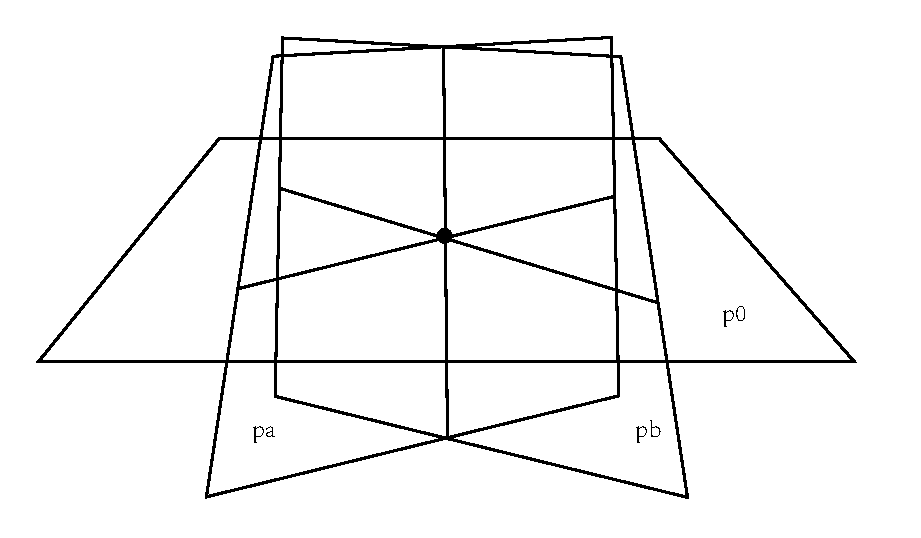
\includegraphics[width=2.5in]{substrates}
\caption{The configuration of two-line-one-plane comparison. $l_a\colon(p_0, p_a)$ and $l_b\colon(p_0, p_b)$ are coplanar in $p_0$. We want to compute $sign(\vec{n}_0 \cdot (\vec{l}_a \times \vec{l}_b))$.}
\label{fig:substrates}
\end{figure}


\section{Exact Intersection Detection}

\label{section:isect}
In this step, intersections between faces are computed through the triangle-triangle intersection test within each critical cell of octree. We adopt M\"{o}ller's intersection detection algorithm \cite{moller1997fast} on account of its efficiency and simplicity. However, because collision detection algorithms are often accompanied by non-robustness problems, a naive implementation may cause unpredictable results when there comes degenerate cases. Therefore, we integrate plane-based geometry representation into M\"{o}ller's algorithm to make it unconditionally robust and exact. In the following, we first make a quick review of M\"{o}ller's algorithm, then discuss the way to integrate plane-based geometry. At last, we talk about how to deal with degenerate case, such as intersecting on points and coplanar case.

\subsection{Vertex-Based Method Review}

\begin{figure}[t]
\centering
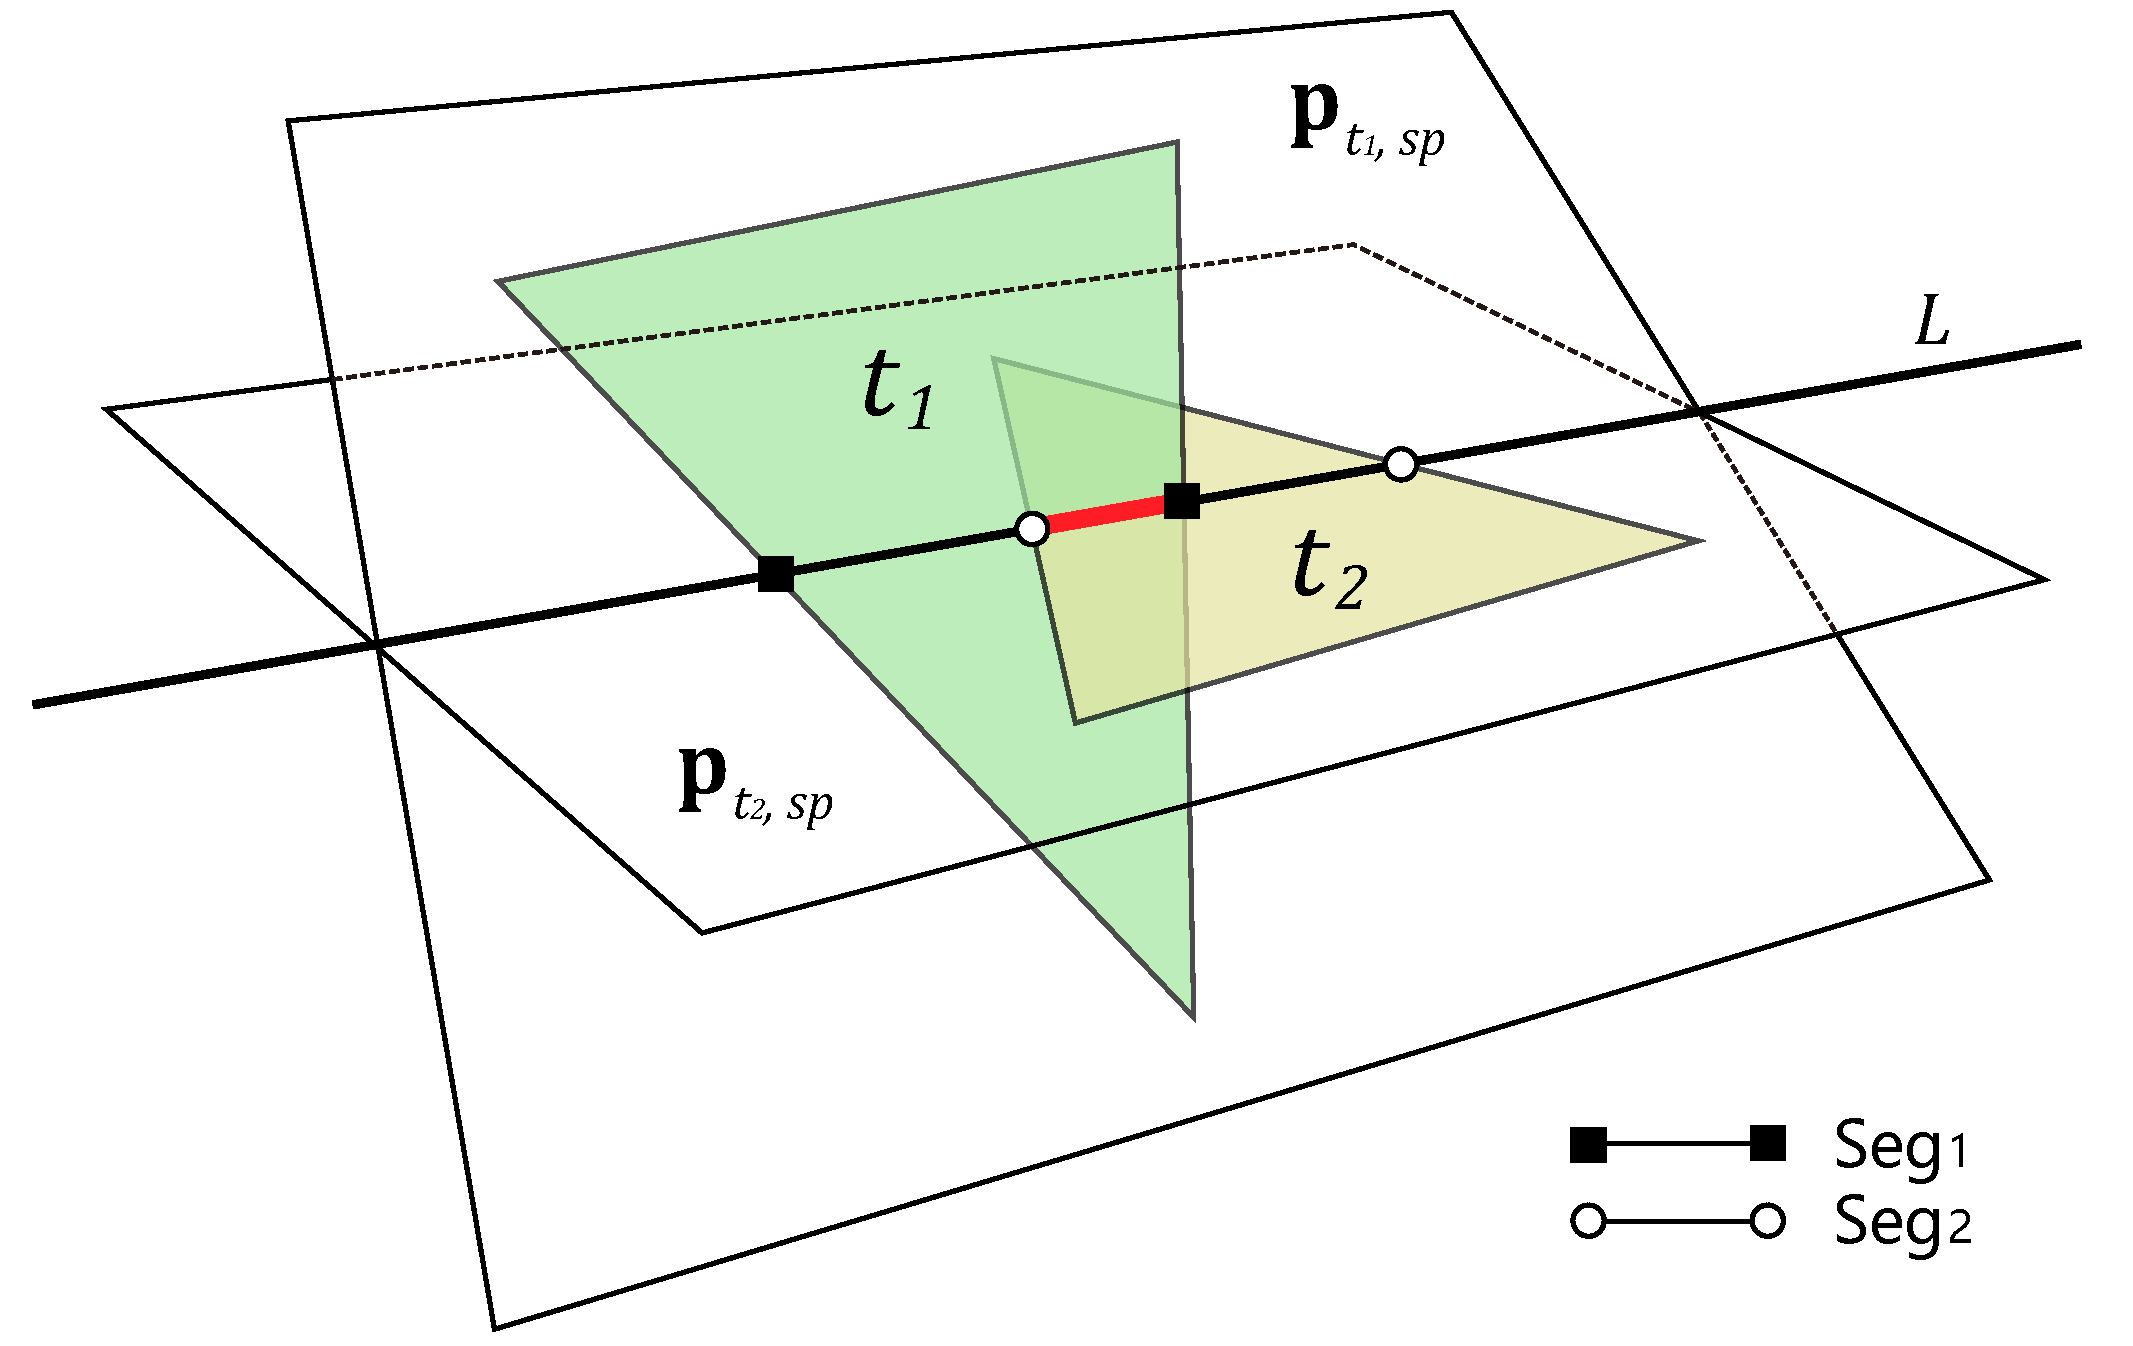
\includegraphics[width=2.5in]{projection}
\caption{$Seg_1$ is the intersection between $p^s(f_2)$ and $f_1$. $Seg_2$ is the intersection between $p^s(f_1)$ and $f_2$. The intersection between $f_1$ and $f_2$, which is the line segment in red, is the overlap of $Seg_1$ and $Seg_2$.}
\label{fig_projection}
\end{figure}


M\"{o}ller's algorithm computes the intersection between two triangles $f_1$ and $f_2$ in three steps (Fig. \ref{fig_projection}).
\begin{itemize}[leftmargin=0.45cm]
\item[1)] An early rejection is performed by testing whether $f_1$ intersects $p^s(f_2)$, the supporting plane of $f_2$. This is a necessary condition of intersection between $f_1$ and $f_2$. If this test is passed, then the same is performed for $f_2$ and $p^s(f_1)$.
\item[2)]The intersection between $f_1$ and $p^s(f_2)$, denoted as $Seg_1$, and the intersection between $f_2$ and $p^s(f_1)$, denoted as $Seg_2$, are separately computed .
 \item[3)]The intersection between $f_1$ and $f_2$ is determined by computing the overlap area of $Seg_1$ and $Seg_2$ .
\end{itemize}

\begin{figure}[t]
  \centering
  % Requires \usepackage{graphicx}
  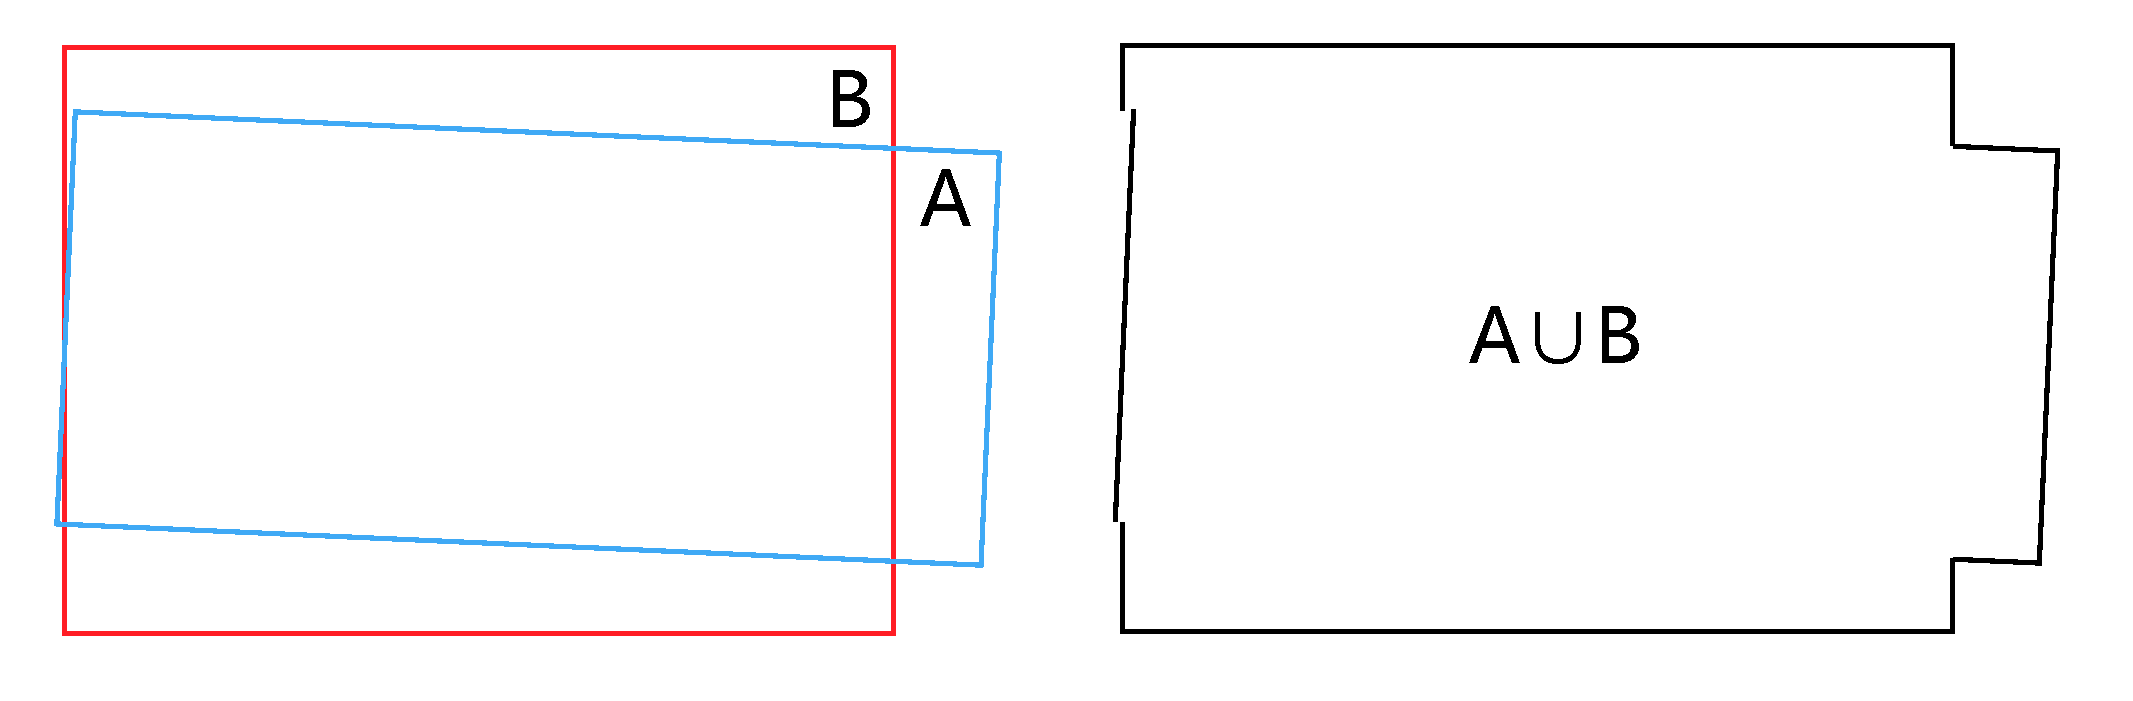
\includegraphics[width=3.0in]{nonrobust}\\
  \caption{The left edges of A and B (\emph{left}) are nearly but not exactly collinear. However, under usual float point arithmetic, they might be judged as collinear causing discontinuous edges in the final result (\emph{right}).}\label{fig:precision}
\end{figure}


Conventional implementations of M\"{o}ller's algorithm use vertex-based geometry, which is neither exact nor robust.  Although implementing M\"{o}ller's algorithm with arbitrary precision arithmetic could make it robust, it is too costly for a large CSG evaluation. Actually, the non-robustness of this algorithm is from geometry \emph{constructions} \cite{bernstein2009fast}, which compute new coordinates of geometry objects based on the known coordinates of existing ones. In M\"{o}ller's algorithm, the coordinates of $Seg_1$ and $Seg_2$ (Fig. \ref{fig_projection}) are computed as intermediate results. We use plane-based geometry to solve these problems by avoiding explicitly computing the coordinates of new vertices.


\subsection{Plane-based Technique Embedding}

\label{sec:embed}
According to the method described in section \ref{sec:convert}, triangle faces $f$ are firstly converted to its plane-based representation: a supporting plane $p^s(f)$ surrounded by three bounding planes $\{p^b_i\ |\  i = 1,2,3\}$. We integrate the plane-based geometry into each of the tree steps of M\"{o}ller's algorithm as following:

\begin{figure}[t]
\centering
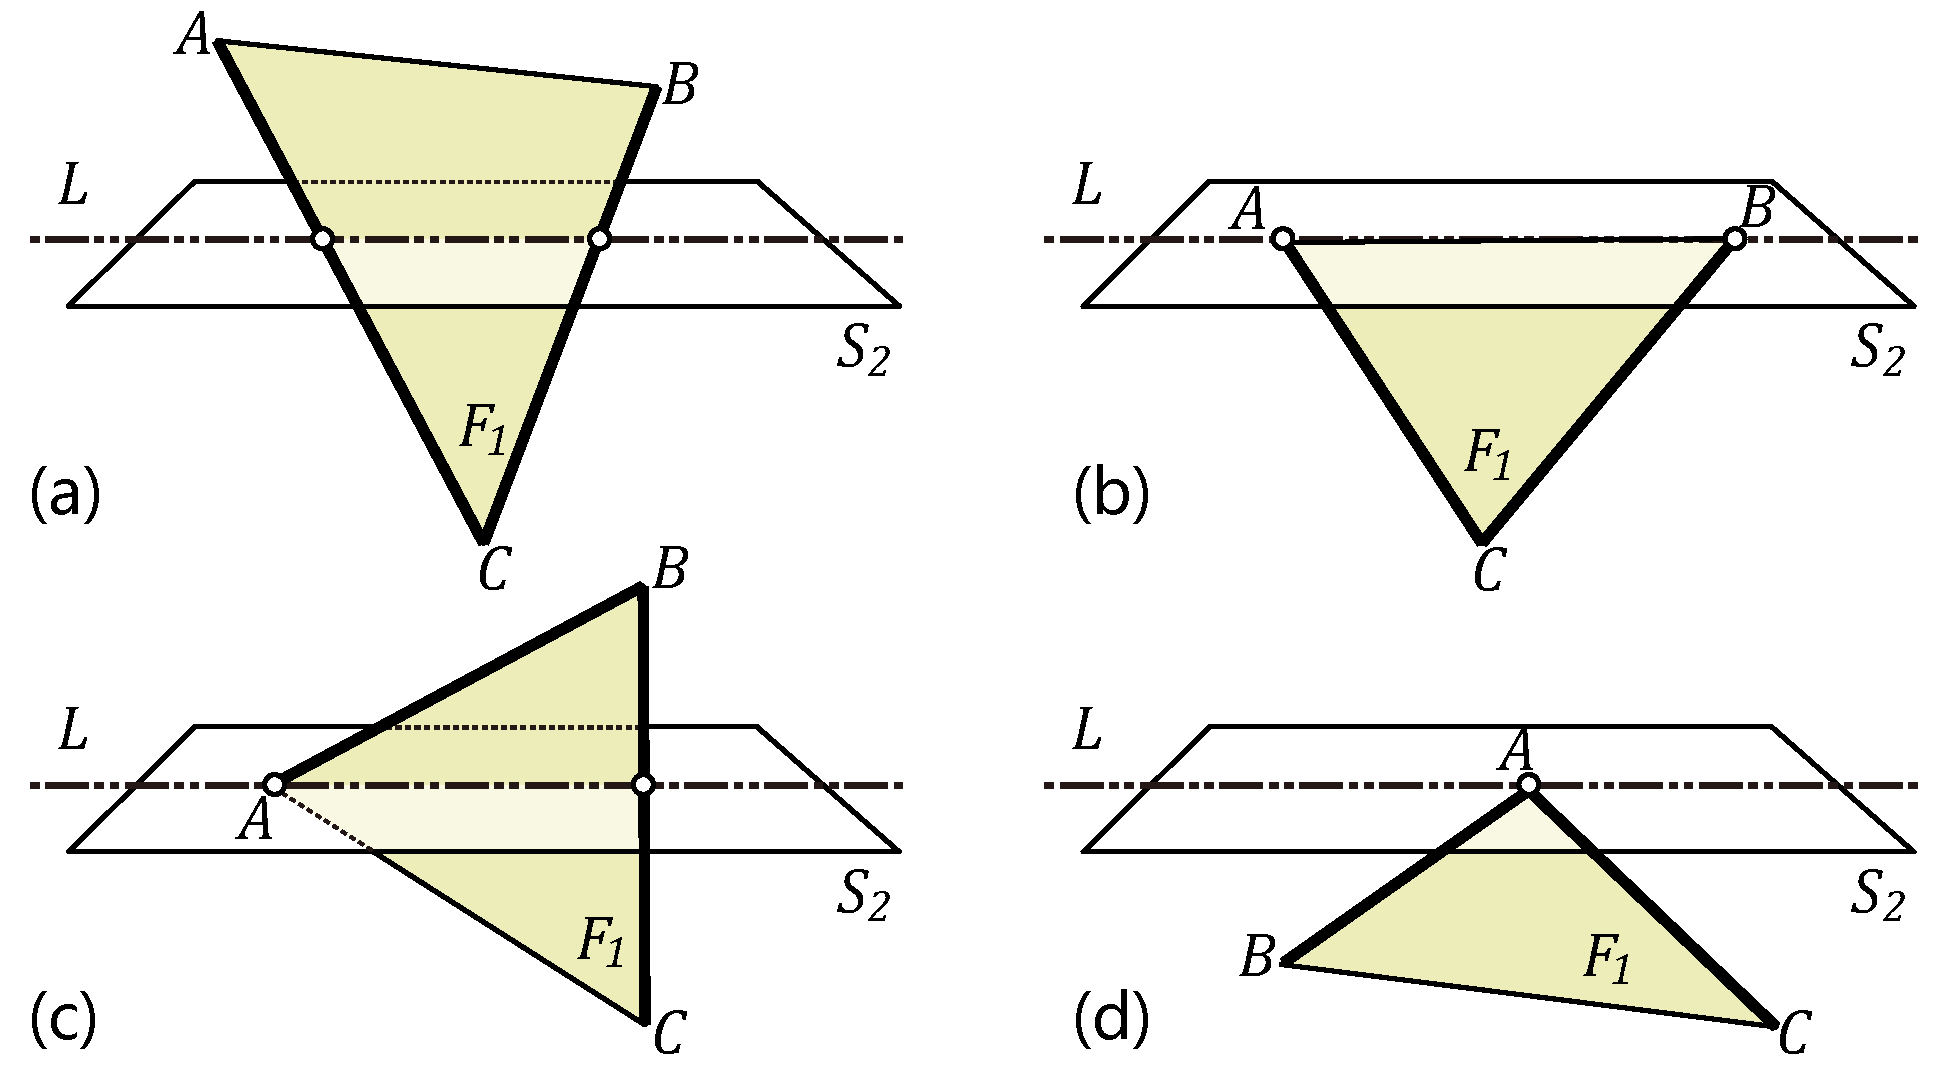
\includegraphics[width=3.5in]{sign}
\caption{We denote the signed distance from point $X$ to plane $S_2$ as $d_X$. All the four conditions of intersection between $F_1$ and $S_2$ (denoted as $Seg_1$) are:  (a) $d_A\cdot d_C<0$, $d_B\cdot d_C<0$; (b) $d_A=0$, $d_B=0$, $d_C\neq 0$; (c) $d_A=0$, $d_B\cdot d_C<0$; (d) $d_A=0$, $d_B\cdot d_C>0$. End points of $Seg_1$ are intersections between $S_2$ and related edge lines of $F_1$ (bold edges).}
\label{fig:isect}
\end{figure}



\begin{itemize}[leftmargin=0.45cm]
\item[1)] The basic routine of the first step is given two faces $f_1$ and $f_2$, computing the orientation of the supporting plane (denoted as $p(f_1)\colon(a, b, c, d)$) of a face with respect to a certain vertex (denoted as  $v_i(f_2)\colon(x, y, z)$) of the other face. That is to compute:
\begin{equation}\label{eq:plane}
sign(ax+by+cz+d).
\end{equation}
Reviewing the discussion of section \ref{sec:convert},  the coordinates of vertices are represented by three L-bit float point numbers.Precisions of the four coefficients of the supporting plane are $(P^\star, P^\star, P^\star, P)$. Here $P$ is defined in equation \ref{eq:precision}, and $$P^\star=P-(L-1)-2.$$ Using the enforced criterion $M \ge P+1$, we find that $M$ bits are enough to perform the predicate of equation \ref{eq:plane}. This allow us to perform the early discard efficiently.
\item[2)]In step 2, the end points of $Seg_1$ and $Seg_2$ are implicitly represented using intersections of plane triples. Take $Seg_1$ as an example. As illustrated in Fig. \ref{fig:isect}, $Seg_1$ are the intersection between $f_1$ and $p_s(f_2)$. Because the edge $e_i(f_1)$ can be represented as $(p^s( f_1), p^b_i(f_1))$, the end points of $Seg_1$ can be represented in the form of $(p^s( f_1), p^s(f_2), p^b_i(f_1))$. In Fig. \ref{fig:isect}, we list all intersection situations between $f_1$ and $p_s(f_2)$, and the corresponding bounding plane $p^b_i(f_1)$ in each situation. Coplanar conditions will be discussed later in section \ref{sec:degenerate}.
 \item[3)] The intersection between $f_1$ and $f_2$ is the overlap area of $Seg_1$ and $Seg_2$. It can be easily computed by comparing the end points of $Seg_1$ and $Seg_2$ along $l$ (Fig. \ref{fig_projection}), where $l$ is the intersection between $p_s(f_1)$ and $p_s(f_2)$. Because end points are all represented using plane triples, we can use the two-line-one-plane comparison discussed in section \ref{sec:substrates} to perform the comparison.
\end{itemize}

\subsection{Intersection Representation}
\label{sec:ir}

// change the title to Indentifying intersections

The output of this stage, or what we call intersection record (IR), is the data structure which organize the results of triangle-triangle intersection test. IR is also the input of tessellation, and is in deep couple with the tessellation method. It is hard to give full idea of why the IR is like that before we introduce our tessellation algorithm. Therefore, in this section, we first give several requirements for IR from tessellation stage, and then discuss the IR structure. To have a comprehensive understanding of IR, readers may need to review this section after finish reading section \ref{sec:tessellation} about tessellation stage.

We recall our definition of Linked Halfedge in section \ref{sec:meshes}, we need to transfer necessary information by IR to tessellation stage for Linked Halfedge construction. For each intersection line segment, we use a five-component vector {\color{red}{$\gamma \colon(T, v_0, v_1, p, C)$}} to describe it. Here, $v_b$ and $v_e$ are the two end points of $\gamma$. Component $f$ is the face where the $\gamma$ lies. Component $C$ is the intersection context, and will be further explained later. Component $p$ is the plane representation of the line where $\gamma$ lies (denoted as $\vec{n}_\gamma$). Normally, line is represented by two planes. However, one of the planes for $\vec{n}_\gamma$ must be $f$'s supporting plane $p^s(f)$, so we just omit it, and use the other plane as the representation for $\vec{n}_\gamma$ .

To illustrate, assume two triangle faces $f_1$ and $f_2$, from primitive $P_1$ and $P_2$, intersect at line segment $\gamma$. Note that there are two versions of $\gamma$ for each of the two faces respectively, denoted as $\gamma(f_1)$ and $\gamma(f_2)$. For $\gamma(f_1)$, $v_b$ and $v_e$ are the two end points of $\gamma$ and $f=f_1$. The representation plane $p$ is $p^s(f_2)$. Note that $p^s(f_2)$ must not be coplanar with $f_1$. The intersection context $C=f_2$ in most cases. It means that, in primitive $P_2$, $\gamma(f_1)$ lies on the face $f_2$. However, sometimes, intersection may lie on the edge, instead of face,  of other primitive. In that case,  the intersection context is an edge, and we discuss such degenerate case in the next section. The situation of $\gamma(f_2)$ is similar we omit the discussion here.

In the Linked Halfedge, there must not be any repetitive vertices in order to reconstruct the correct topology. Therefore, repetitive vertices elimination must be performed. Checking whether there are coincident points in a global scope can be quite inefficient. Our implementation use a localized scheme that store the reference of intersection vertices into their corresponding geometry location, like edges and faces. Therefore, coincidence detection performed within the geometry elements and repetitive vertices elimination can be very fast.

\subsection{Degenerate Cases}
\label{sec:degenerate}

Assume there are two faces $f_1$ and $f_2$ from primitive $P_1$ and $P_2$ respectively. These two faces intersect on line segment $\gamma$, which has two versions of IR $\gamma(f_1)$ and $\gamma(f_2)$ for the two faces respectively. Without loss of generality, we only discuss the configuration of $\gamma(f_1)$, as $\gamma(f_2)$ can be figured out similarly. We classify all degenerate cases into three categories by the dimension of intersection. Each of them is discussed separately in the following.

Before we go into details, there are three principles that we follow to solve degenerate cases:
\begin{itemize}
\item We want our method be unconditional robust and exact, so all degenerate cases should be well handled (completeness).
  \item To control the complexity of tessellation, we want degenerate cases to be invisible to tessellation, that is, degenerate cases have the same format of output, in our method, IR, as non-degenerate cases (invisibility).
  \item we want the outcome of tessellation be as simple as possible. That is, intersection line segments that will not help tessellation, if recognized, are disposed (concision).
\end{itemize}
The criterion of whether an intersection help tessellation is by its necessity: if the intersection is not presented, whether some faces from the linked halfedge will cross the boundary of primitives. The word 'cross' do not only include the situation that a face is partly outside and partly inside of a primitive, but also can mean that a face is partly inside (outside) and part on the boundary of the primitive.



\subsubsection{Intersects on point}
\label{sec:ipoint}
When two triangles intersect on a single point, there are two different conditions (Fig. \ref{fig:isolated}), depending on whether the point is isolated. If the point is isolated, it means that there is no other intersection line segment sharing the point. This condition may cause non-manifold surface because of the singularity of the isolated intersection point. Also, isolated intersection point will not affect the tessellation of the intersection face. On the other hand, if the intersection point is not isolated, there must be other intersection line segments that contain the point, thus the point will be introduced at least twice. Therefore, no matter which condition it is, when two triangle faces intersect on point, we can just omit this intersection and this will not affect the correctness of the final topology.

\begin{figure}[t]
\centering
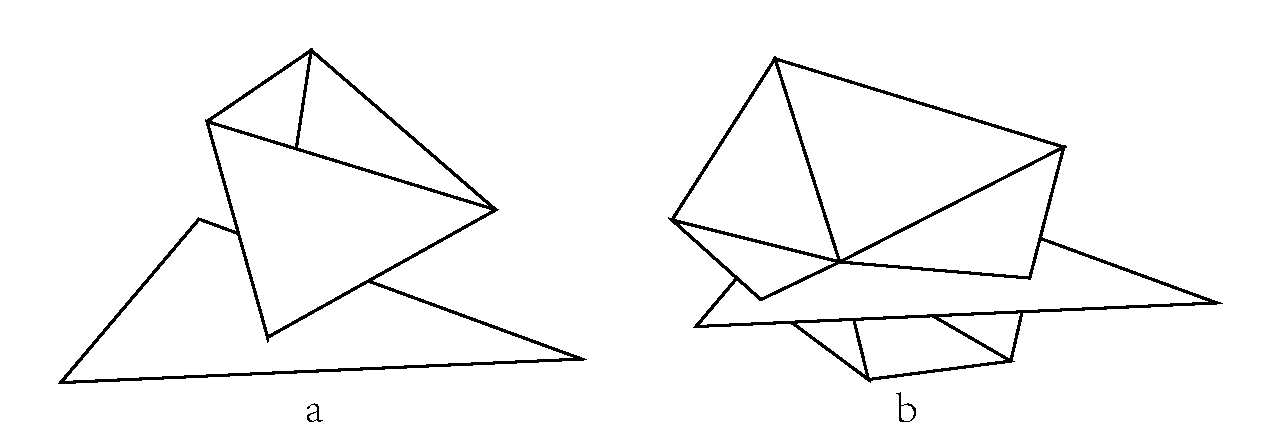
\includegraphics[width=3.5in]{isolated}
\caption{Two situations of point intersections. (a) The intersection point is isolated, and there is no adjacent intersection line segment. This situation may cause non-manifold surface in Boolean operation. (b) The intersection point is not isolated. The intersection point can be introduced by other face pairs during intersection tests.}
\label{fig:isolated}
\end{figure}


\subsubsection{Intersects on face edges}

// intersect on face edges does not create new line segments, it is part of the edges from other meshes, and will to be duplicated.


// whose edge? need to be further explained and better defined. an edge intersection divide edge in a triangle and will be duplicated in the other


When intersection line segment lies on an edge (Fig. \ref{fig:twin}). we call it as \emph{edge intersections}. There are generally two kinds of edge intersections. If $\gamma$ lies on the edge of $f_1$ or $f_2$, but inside of the face of the other one, then we called it as edge-face intersections. If $\gamma$ lies on the edges of both $f_1$ and $f_2$, we call it as edge-edge intersections. When there is edge-face intersection, we treat it as the intersection of three faces $f_1$, $f_2$ and $f_1^\star$ (or $f_2^\star$). When there is edge-edge intersection, we treat it as the intersection of four faces $f_1$, $f_2$, $f_1^\star$ and $f_2^\star$. The $f_1^\star$ (or $f_2^\star$), known as \emph{companion face},  is the neighboring face which shares the intersection edge with $f_1$ (or $f_2$). In this way, we avoid repetitive insertion of the same edge intersections, since the companion faces share the same intersection with its neighborhood $f_1$ or $f_2$.

\begin{figure}[t]
\centering
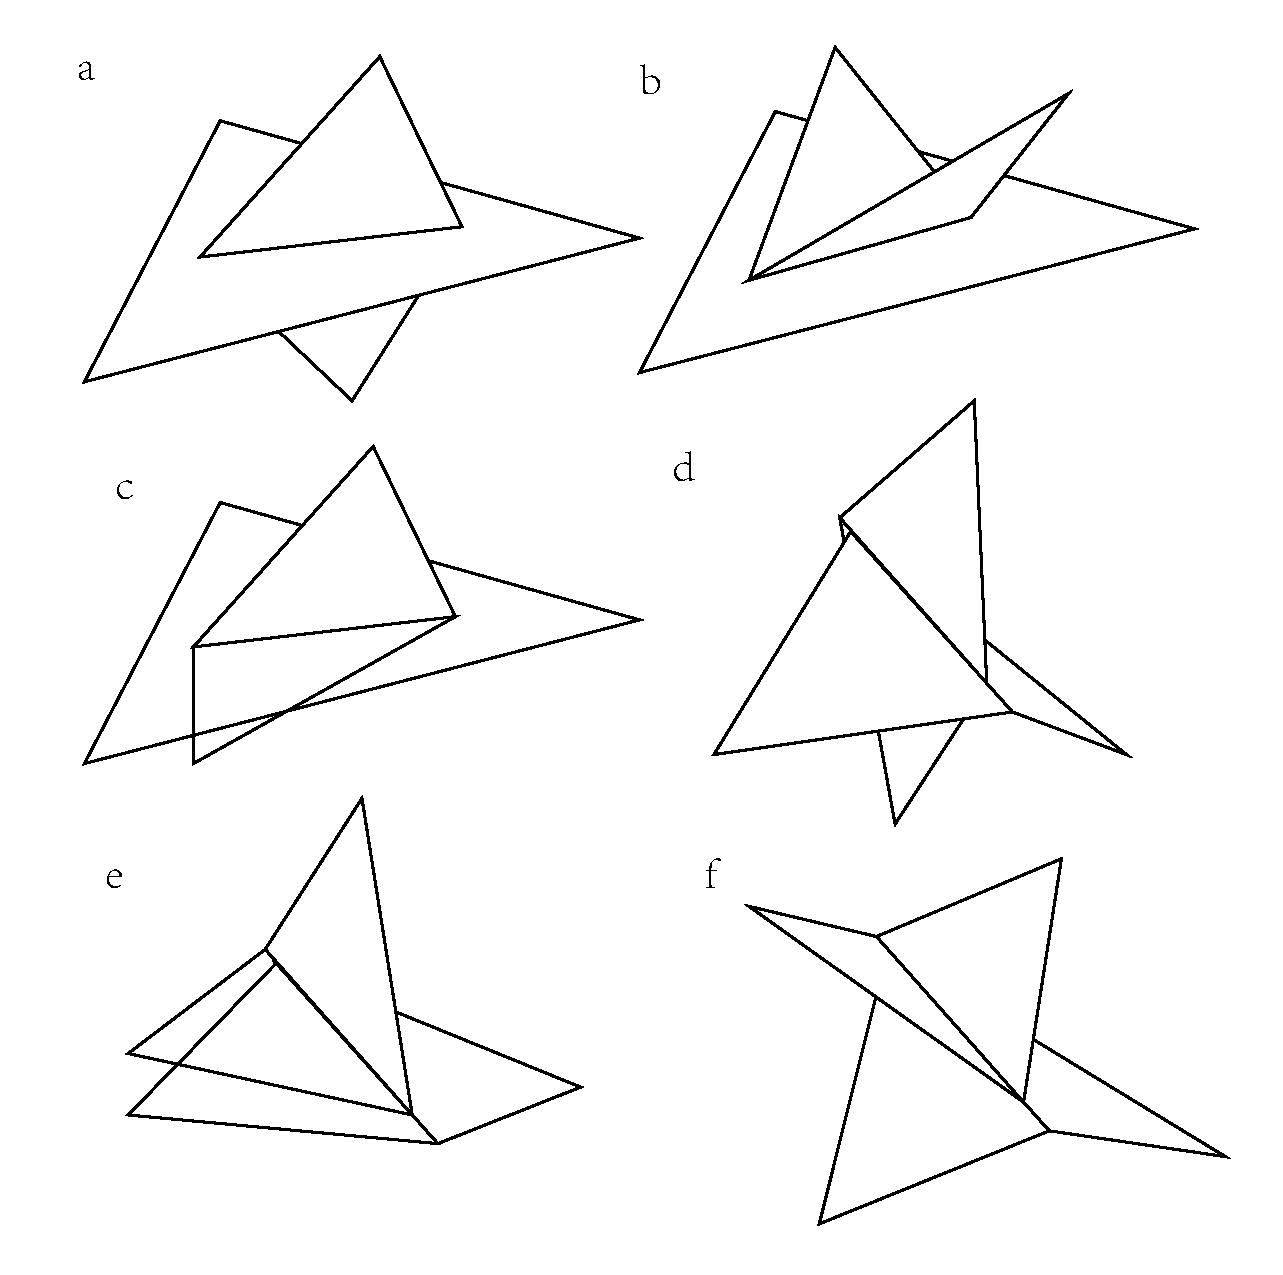
\includegraphics[width=3.5in]{twin}
\caption{Six situations of edge intersections. The first three subgraphs are edge-face intersections. The last three ones are edge-edge intersections. (a) Triangles are located in two sides, cross condition. (b) Triangles are located in the same sides, invalid condition. (c) One of the triangles are coplanar, coplanar condition. (d) Double twin intersections, cross condition. (e) Double twin intersections, coplanar condition. (f) Double twin intersections, coplanar condition.}
\label{fig:twin}
\end{figure}

Both edge-face and edge-edge intersection can be further classified into three subclasses by the location of companion faces---cross condition, coplanar condition and invalid condition. We first consider edge-face intersection. If $f_1$ and $f_1^\star$ are on the same side of $f_2$, it is cross condition. If they are on the same side, it is invalid condition. If $f_1^\star$ is coplanar with $f_2$, it is coplanar condition. Consider the cross and coplanar condition. For $f_2$, the IR is the same as the common situation, except that the intersection context is an edge. For $f_1$ and $f_1^\star$, they have to share the intersection line segment, while the intersection context is $f_2$.  However, when there is invalid condition, we should not record the intersection for the similar reasons of isolated point intersection (section \ref{sec:ipoint}).

The handling of edge-edge intersection is similar with edge-face intersection. The difference is that the intersection contexts are edges for both $f_1$ and $f_2$. We still can classify edge-edge intersection into three subclasses by the relative location of companion faces. There is one difference, though, that in edge-face intersection, we compute on which side of $f_2$ the companion face $f_1^\star$ lies, and compare with $f_1$. However, in edge-edge intersection, we have to consider the space split by both $f_2$ and $f_2^\star$ instead of only $f_2$.  Similar with edge-face intersections, we record the intersection of cross and coplanar condition, while omit the invalid condition for concision and also topology correctness.

\subsubsection{Coplanar cases}

\begin{figure}[t]
\centering
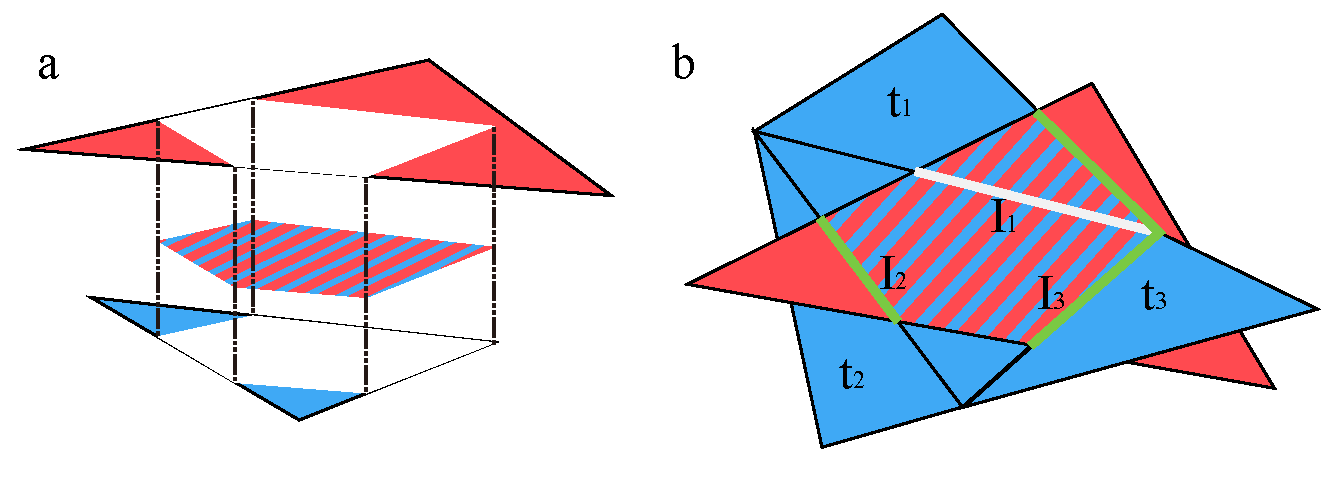
\includegraphics[width=3.5in]{coplanar}
\caption{a) Coplanar cases and the b) the possible configurations of the companion faces. In any configurations, their is no need to record the intersection of coplanar cases.}
\label{fig:coplanar}
\end{figure}

Consider two triangle faces $T_1$ and $T_2$ intersect within a common plane. Both $T_1$ and $T_2$ will divide each other into two areas---the overlapped area and the exclusive part (Fig. \ref{fig:coplanar}). Obviously, if we tessellate both $T_1$ and $T_2$ according to the boundary of overlapped area, we can guarantee that the tessellated meshes will not cross the boundary of any other meshes. In fact, many methods \cite{feito2013fast} claim that it is important to tessellate faces according to the 2D-intersection result. We will show that this is not necessary in our method. We do not care whether $T_1$ and $T_2$ really intersect in 2D. We simply omit all coplanar cases, treating them as they do not intersect. This simplify our intersection test, making it more robust and fast (coplanar cases can be usual in a CSG of artificial object), while doing no harm to the correctness of our method.

The key observation is that coplanar cases do not create new edges, just like edge intersection in the last section. The difference is that in a non-coplanar case, there is only one edge intersection. In a coplanar, there are at most three intersections. Therefore, we can decompose it into three edge intersections and record each edge intersection independently. However, there is a better way that we do not process them at all. This is because there is companion face, like $T_1^*$, in edge intersection. If $T_1^*$ is not coplanar with $T_2$, then we can solve the intersection between $T_1^*$ and $T_2$ in a 3D way, which is the case in Fig \ref{fig:twin}(c). On the other hand, if $T_1^*$ is coplanar with $T_2$, we instantly know that both sides of shared edge $e(T_1, T_1^*)$ have the same indicator $\lambda_1$, which imply that this intersection is not necessary for tessellation and we can omit it by the principle of concision. In sum-up, we do not need to handle with coplanar intersection cases.

\section{Deferred Tessellation}

{\color{red}{red alert start}}

\label{sec:tessellation}
This is the step to tessellate input meshes with intersections, outputting linked halfedge. We called this stage as deferred tessellation because it happens until we collect all necessary intersections. For this problem, Ogayar-Anguita et. al. \cite{ogayar2015deferred} try to use Constrained Delaunay Triangulation (CDT) to solve, as the intersections is naturally the constraints and triangle faces is naturally a convex zone. It works fine for Boolean operation of two primitives. However, when there are more than two primitives, simply applying CDT covers the complexity of tessellation. The major problem here is that the intersections may be \emph{irregular}. The definition of regular intersection is that it does not cross or overlap with other intersections. In CSG cases with more than two meshes, irregular intersections can introduce new vertex, split original intersection line segments. However, most CDT algorithms \cite{chew1989constrained}, or even just constrained triangulation [Computational geometry: an introduction] require that constraints do not cross each other, and will cause topology deficiency if not satisfied.

To solve these problems, we first refine the intersections and eliminate any irregular intersections. When all intersections are regular, we can directly use CDT to tessellate. However, 2D constrained triangulation algorithm \cite{chew1989constrained} [Computational geometry: an introduction] require cross detection between arbitrary connections of vertices, coordinates projection, which is hard to exactly performed using plane-reps geometry. Therefore, we develop a new tessellation algorithm using only plane-based geometry, ensuring topology correctness and unconditional robust. We first organize intersections into single face scope, generating an intermediate data structure---\emph{Tess-graph}. Then we tessellate each face by subtract sub-faces from its corresponding Tess-graph. In compensate, we do not guarantee the faces of the final mesh are triangles, leaving the flexibility to post-processing.

\subsection{Eliminating Irregular Intersection}

Regular intersections are guaranteed when there are only two meshes, because the surfaces of primitives are all without self-intersection. However, when there are more than two primitives, this constraint can be violated. In the view of intersection detection, it is not enough to find all intersection vertices by only triangle-triangle intersection test. This is because in such case, the new vertex can be introduced not only by intersection between edge and plane, but also by intersections of three planes, which involves more than two faces.

Intersection refinement is performed in a local scope. For each face, we detect irregular intersections by intersection test between pairs of intersections. Because primitive meshes are not self-intersected, we only check intersections between intersections made by different meshes. Face intersecting only one other mesh do not need refinement, since they do not have such intersection pairs.

Using plane-based representation, whether two intersections intersects each other is determined by predicate of orientation of plane against a point. For example, we want determine whether $\lambda_1$ and $\lambda_2$ intersects. Using the notation of section \ref{sec:ir}, we perform the test by checking whether $v_0(\lambda_1), v_1(\lambda_1)$ are on two sides of $p(\lambda_2)$ and whether $v_0(\lambda_2), v_1(\lambda_2)$ are on two sides of $p(\lambda_1)$. If yes, $\lambda_1$ and $\lambda_2$ intersects and introduces new intersection vertex $v_{new}$, which is the intersection of $p(\lambda_1), p(\lambda_2)$ and the supporting plane of $T(\lambda_1)$. The new vertex $v_{new}$ should be added into both $\lambda_1$ and $\lambda_2$ as a segment point. Since there may be more than one segment point added into a certain intersection during the whole test, we do not divide the intersection until all intersection pairs are tested.

Degenerate cases are when the two intersections intersect on one of the end points or are collinear. In the first condition {\color{red}{Fig. ??(a)}}, there is no new vertex generated and only one of the intersection needs splitting. The collinear case {\color{red}{Fig. ??(b)}} is intersection in 1D and are tested exactly by two-point-on-line comparison between the end points of intersections. If there is intersection between them, it should be straightforward to figure out the segment points for each intersections.

After all segment points are found, the related intersections have to be split. For a certain intersection, we sort the segment points by two-point-on-line comparisons and subtract child intersections along the direction of their father one by one. The representation of the child intersections should be the same with their father except the coordinate components $v_0$ and $v_1$. So far, we guarantee that all refined intersections need not be further divided as the potential edges of the Linked Halfedge. However, if there are collinear cases, there will be coincident child intersections from different fathers. We choose to resolve them in Tess-graph. If CDT is chosen instead of Tess-graph, coincidence can be handled like-wise.

\subsection{Tess-Graph}

So far, intersections are only loose data that store the coordinates and neighbouring information. To perform tessellation and extract sub-faces, we need to organize them to reveal the topology. We use Tess-graph for this purpose. A Tess-graph is the graph description of the tessellated face topology. For each face to be tessellated, we construct a Tess-graph according to the refined intersections. The final Linked Halfedge merges both the original topology and the intersections in the same representation. And the construction of Tess-graph is the first step towards such uniformity. By only nodes and connections, it represents both the intersections and the original boundary of triangle face. This reduces complexity of the following processes and allowing them to be simple and fast.


Nodes of Tess-graph represent vertices and store the coordinates of them. Connections are nondirectional, represent edges in Linked Halfedge, storing the I-rep if it is coincident with an intersection. Sometimes, there will be more than one coincident intersections and all I-reps have to be stored. Construction of Tess-graph from I-rep is straightforward except one thing: we have to merge face boundary with the intersections lies on the face boundary {\color{red}{Fig}}. This lead to an extra step beforehand. For each edge boundary of face, we treat it as pseudo-intersections with only coordinates information, and perform collinear intersection test with all intersections lies on it, splitting it by corresponding segment points.

\subsection{Extracting Sub-faces}

The difference between a graph and a mesh surface is that there is no concept of face in graph. In this step, we extract faces from Tess-graph to construct Linked Halfedge.

First, We classify connections of Tess-graph into two types: connections on face boundaries as \emph{boundary connections} and connections inside face as \emph{inner connections}. In the view of halfedge data structure, inner connections represent two opposite halfedges but boundary connections represent only one. We add an attribute for each connection to identify their directions, and thus we get a directed version of Tess-graph. A sub-face is a halfedge loop on the directed Tess-graph. Extracting faces are process of searching for valid loops which meet certain geometry constraints. After all faces are extracted, all halfedges of directed Tess-graph should be used exactly once.

There two geometry constraints for valid loops. First, the direction of loops should be coherent with the face normal, counter-clockwise for example. Second, consecutive halfedges on the loop should be angle adjacent, which means there is no other halfedges between the angle contained by these two halfedges {\color{red}{Fig.?}}. To meet these constraints, we sort the halfedges counter-clockwise for each nodes with more than two halfedges starting from them. This is implemented by using the divide-and-conquer framework of quick sort. During each recursion, we pick a random halfedge and split the rest into two sets according to the sign of two-line-on-plane comparison. To make the results of two-line-on-plane comparisons coherent, we assume that for each halfedge $h_i$, the normal directions of its plane-rep, denoted as $\vec{n}(h_i)$, meets the following criterion:
\begin{equation}
(\vec{n}(h_i) \times \vec{n}_0) \cdot \vec{l}(h_i) > 0,
\end{equation}
where $\vec{n}_0$ is the normal of the face, and $\vec{l}(h_i)$ is the direction of $h_i$. The plane-rep of halfedge can be inherited from the corresponding connections from the undirected Tess-graph. Since we {\color{red}{guarantee that each connection has a plane-rep //need insert//}}, sorting can be exactly and fast performed. After connections are sorted in each nodes, we can know which connections are adjacent and what is the right direction during the loop search.


\section{Face Classification}

\label{sec:classification}
This stage traverses all candidate faces in the Linked Halfedge, and classifies which of them belong to the final mesh. Classification is done by evaluating the indicator vector of each face {\color{red}{(indicator vector?)}}. During this process, we take advantage of plane-based representation to ensure unconditional correct classification. In addition, since we maintain the intra-primitive geometry connectivity and inter-primitive geometry connectivity in Linked Halfedge, we can utilize the space coherence of face indicator vectors to accelerate this process.

In this section, we will first give an overall framework of face classification, and then introduce how to classify each individual face. At last, we discuss how to accelerate this process by caching intermediate results.

\subsection{Framework}

The space coherence of indicator vectors means neighboring faces could share the same indicator vector, or most components of indicator vectors. For example, given two neighboring faces $t_1$ and $t_2$, indicator vectors $\Lambda(t_1)$ and $\Lambda(t_2)$ would often be the same. Only when there is boundary of some meshes, say $P_k$, on the shared edge $e(t_1, t_2)$ and split $t_1$ and $t_2$ in two sides, the corresponding components $\lambda(t_1, P_k)$ and $\lambda(t_2, P_k)$ can be different. And other components of $\Lambda(t_1)$ and $\Lambda(t_2)$ will remain the same. If we can compute the indicator changes between neighboring faces efficiently, we can start from a single face with a indicator vector as the seed, propagating to all faces with geometry connectivity, reusing indicator vectors according to the spatial coherence and classifying faces very fast.


Fortunately, in the Linked Halfedge, it is straightforward to know whether $\lambda(t_1, P_k)$ and $\lambda(t_2, P_k)$ are different, because it means $e(t_1, t_2)$ will be on the boundary of $P_k$, and there will be corresponding I-reps stored on $e(t_1, t_2)$. In addition, both $\lambda(t_1, P_k)$ and $\lambda(t_2, P_k)$ can be computed efficiently according to the I-reps (details in Section \ref{sec:individual}). We outline our classification method in Algorithm 1.

\begin{algorithm}
\caption{Fast Face Classification}
\label{code:floodfill}
\textbf{Input: } Linked Halfedge structure $\Omega$

\textbf{Output: } Classification of each face $f(\Lambda(t_i)), t_i \in \Omega$


\begin{algorithmic}[1]
\State Select a proper seed face $t_s$
\State Compute the first indicator vector $\Lambda(t_s)$
\State \Call{propagate} { $t_s$ , $\Lambda(t_s)$}
\State
\Function{propagate}{ $t_c$ , $\Lambda(t_c)$}
    \State Compute $f(\Lambda(t_c))$
    \For {each neighboring face $t_i^c$}
        \If {there are I-reps $\{\gamma_k\}$ on $e(t_i^c, t_c)$}
            \State Compute $\Lambda(t_i^c)$ using $\Lambda(t_c)$ and $\{\gamma_k\}$
            \State \Call{propagate} { $t_i^c$ , $\Lambda(t_i^c)$}
        \Else
            \State \Call{propagate} { $t_i^c$ , $\Lambda(t_c)$}
        \EndIf
    \EndFor
\EndFunction
\end{algorithmic}
\end{algorithm}

\subsection{Seed Indicator Vector}

Our classification method starts from computing the seed indicator vector using point-in-polyhedron test \cite{ogayar2005point}. Conventionally, the barycenter of the face is used for the test to compute the indicator vector of the whole face. This is because the whole face is classified as a whole, and every inner point will have the same indicator vector. However, the coordinates of the inner points cannot be exactly represented by float point numbers, which may lead to wrong predicates, especially when it is an on-boundary case. Therefore, we use the original vertices, whose exact coordinates are known, for point-in-polyhedron test. For this reason, only tessellated faces with at least one original vertex can be the seed face. The point-in-polyhedron test is guaranteed to be exact. On the other hand, efficiency is not so important as there will not be many such tests. If ray-trace algorithms (e.g., \cite{frisken2002simple}) are used, the octree constructed during space division can be used for acceleration \cite{havran1999summary}.

However, using point on the boundary instead of an inner one has another problem. Given a face $s$ (may not be triangle) and one of its vertex $v_b^i(s)$, the vertex indicator $\lambda(v_{i}(s), P_k)$ may cause ambiguity to deduce the face indicator $\lambda(s, P_k)$. In {\color{red}{Fig. ?}}, $\lambda(v_b^1(s), P_k) = on$, then $\lambda(s, P_k)$ can be any of the four conditions. We solve this problem by trying other vertices in $s$ for the ambiguous components. If all vertices indicators are $on$ and the ambiguity still cannot be resolved, the current face is not proper for being the seed and select a new one instead.

\subsection{Fast and Exact Face Classification}

\label{sec:individual}

Feito et. al. \cite{feito2013fast} had noticed that intersection neighborhood can be used for fast classification of faces around that intersection. According to their method, faces adjacent to intersection have neighbors from other primitive(s) that define the position and orientation for each other, by which the indicators are determined. However, Feito et. al. did not give detail description of how to implement an exact and robust classification. Their implementation of using vertex coordinates may have problems for the degenerate cases. Because geometry connectivity is used, local incorrect classification can be spread to the neighborhoods, leading to errors in wide ranges.

{\color{red}{fdafdafdsfafdfadsfa}}

During flood-filling, we propagate the indicator vector of the current face $f_0$ to its neighboring faces, which have shared edges with the current face. If one of shared edges has intersection context $C_{I_v \mapsto A}$, it means the indicator of primitive $A$, denoted as $i_A$, could be different for the corresponding neighboring face $f_i$. In this section, we will show that $C_{I_v \mapsto A}$ is enough to compute the new $i_A$ for $f_i$. We only discuss the condition that $f_i$ is a triangle in the following. However, $f_i$ may not be triangle, not even a convex polygon. In these conditions, we can select a triangle subset of $f_i$ to represent $f_i$, since $f_i$ is guaranteed to be classified as a whole.

We develop an exact and robust classification method based on the idea of using intersection neighborhood information. The intersection neighborhood is abstracted into two situations of intersection context (section ??). To make a clear description, we denote the three corners of neighboring face $f$ as $v_0^I$, $v_1^I$, $v_2$, where the superscript means the vertex lies on the intersection line segment $I$ with intersection context $C_{I \mapsto A}$. In the first situation, the intersection $I$ lies on the face of primitive $A$. That is, $C_{I \mapsto A} = f_x^A$. To calculate indicator $i_A$ for $f$, we only need to decide on which side of $f_x^A$ the current  face $f$ lies. Any sample point on $f$ except those on $I$ can be used for this predicates. As we can get the exact coordinates of corners, we choose $v_2$ to compute $i_A(f)$.

If $I$ lies on edge of primitive $A$,  the intersection context is face pair: $C_{I \mapsto A} = (f_p^A, f_q^A)$. This situation is a little more complex that we cannot decide $i_A$ until we check the orientations of both $f_p^A$ and $f_q^A$. To correctly classify $f$, we first build BSP structure using $f_p^A$ and $f_q^A$ [?], and then determine the space indicator $i_A(v_2)$ by the BSP. As coordinate of $v_2$ and all the planes can be exactly computed, the classification is exact. The indicator of the face $i_A(f)$ should be the same as $i_A (v_2)$. It is because under a BSP structure with only two division planes, any sample point on $f$ except those on $I$ has the same $\lambda_A$ (Fig. ??).


\subsection{Caching Evaluation Results}

If the CSG tree is large, with tens of, or even hundreds of nodes, computing $\lambda_\Phi(f) = \Phi(\vec{\lambda}(f))$ for every face can be costly. Considering the space coherence of indicator, we use cache techniques --- by storing the evaluation result of $\Phi$ --- to save the computation time.

The most simple cache strategy is final result cache. We know indicator vector $\vec{\lambda}$ will not change if there is no intersection context during spreading. That means the final classification $\lambda_\Phi$ will not change, too. Thus, those faces sharing the same $\lambda$ can be classified as a whole.

Also, we can also do intermediate result cache. It should be noticed that $\Phi(\vec{\lambda}(f))$ can be simplified if some components of $\vec{\lambda}$ is fixed. For example, assume we have a Boolean expression $M_1\cup (M_2\cap M_3-M_4)$. Given the values of two indicators $\lambda_1(x)=out$, $\lambda_2(x)=in$, the expression can be rewritten as $out\cup (in\cap M_3-M_4)$. Using the combination rules we can simplify the expression as $M_3-M_4$. This fact is important because for a large CSG tree, a certain primitive, denoted as $M_x$, often only intersects with a few other primitives $\Theta= \{M_{n_1}, M_{n_2}, \cdots, M_{n_k}\}$. That means all the faces in $M_x$ has the same indicators for the primitives not in $\Theta$. Therefore, we can first determine these fixed indicators and simplify the Boolean function $\Phi$ into a simpler one $\Phi_{M_x}$, and then use $\Phi_{M_x}$ to compute the final indicator for each faces.


\section{Implementation}

\vspace{0.5em}
\textbf{Generate Seed Indicator Vector.} Our method of generating the first indicator vector will fail on extreme conditions when each face in Linked halfedge is coincident with more than one primitive face (e.g., the union of the same mesh). In order to be robust, we use the face barycenter with high-precision coordinates for the point-in-polyhedron test to generate the seed indicator vector after several failures of choosing a proper seed face.

\vspace{0.5em}
\noindent \textbf{Generate Seed Indicator Vector.} Our method of generating the first indicator vector will fail on extreme conditions when each face in Linked halfedge is coincident with more than one primitive face (e.g., the union of the same mesh). In order to be robust, we use the face barycenter with high-precision coordinates for the point-in-polyhedron test to generate the seed indicator vector after several failures of choosing a proper seed face.

\section{Summary}

In this paper, we proposed a novel method to evaluate CSG with triangular mesh primitives. It is able to efficiently perform non-incremental evaluation of large CSG with massive faces. The key idea of our approach is to use the local coherence of face space labels to accelerate face membership classification. A two-level grouping framework is developed to group neighboring faces together and thus space labels can be shared within each group. This scheme saves much time for space label computation, which is often very time-consuming for conventional Boolean evaluation algorithms. Additionally, in order to be robust, plane-based geometry computation is introduced into the intersection computation step of our approach. Experiments have verified the proposed approach is more efficient than the state-of-the-art techniques while retaining robustness and stability. We will further investigate the robust tessellation in future.



\appendices



%\newpage
\bibliographystyle{IEEEtran}
\bibliography{IEEEabrv,citation}


%\newpage

\begin{IEEEbiography}[{\includegraphics[width=1in,height=1.25in,clip,keepaspectratio]{rui}}]{Rui Wang}
is currently a postgraduate student at the Department of Computer Science and Technology, the Shanghai Jiao Tong University. His main research interests include real-time computer graphics and virtual reality applications.
\end{IEEEbiography}

% if you will not have a photo at all:
\begin{IEEEbiography}[{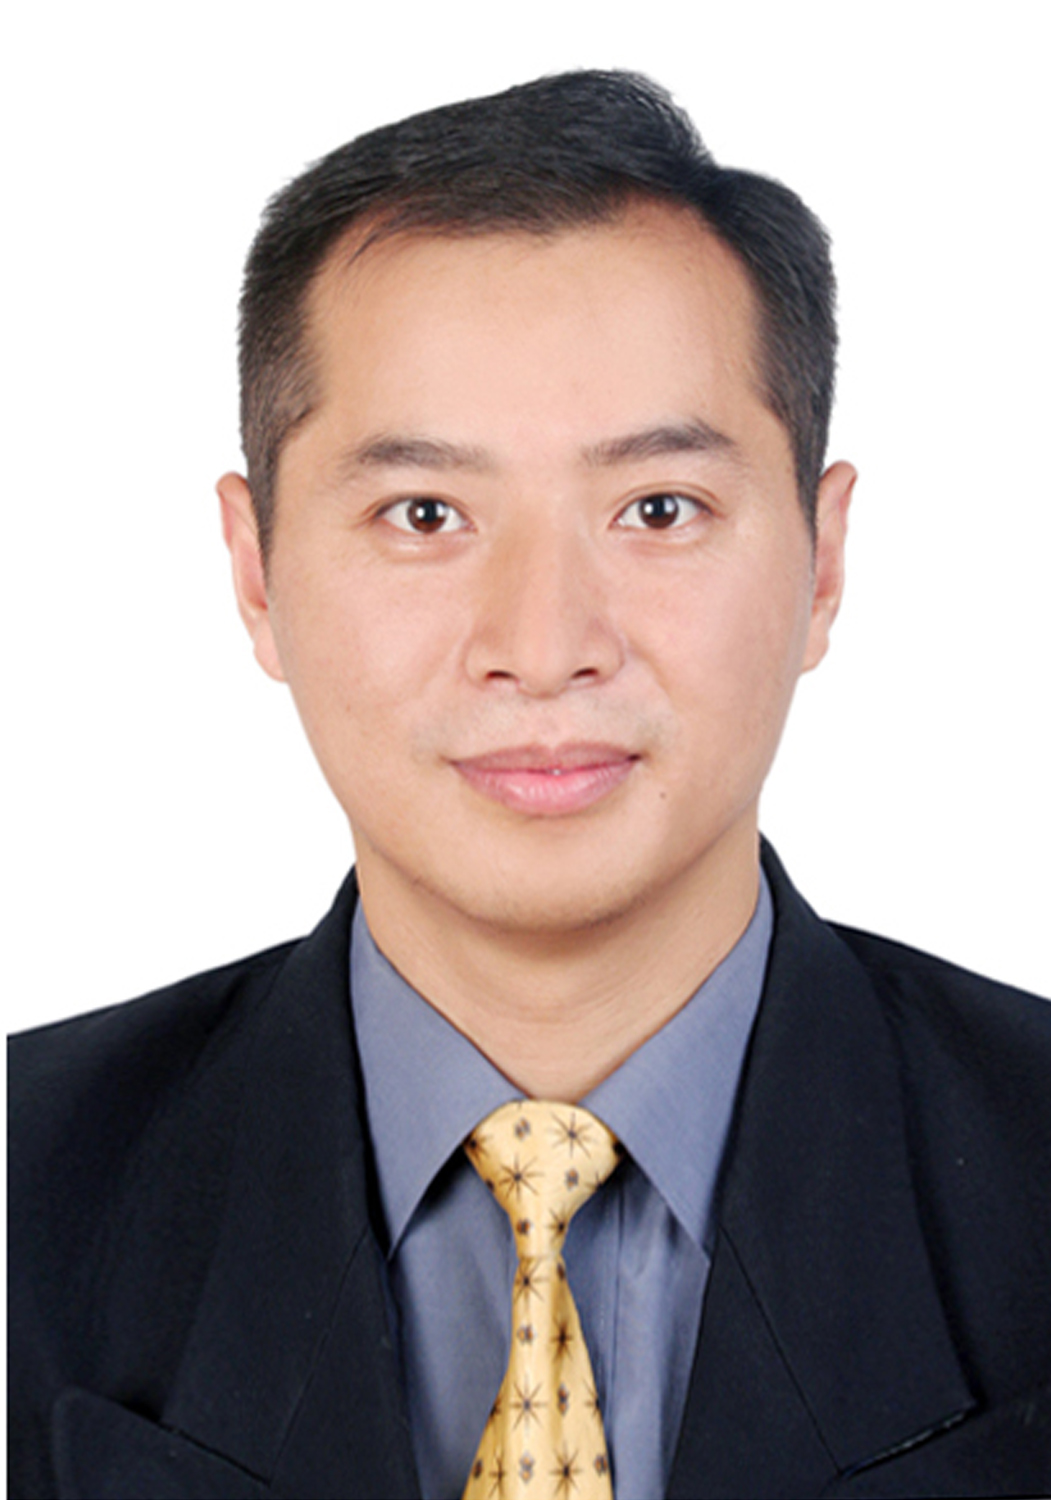
\includegraphics[width=1in,height=1.25in,clip,keepaspectratio]{xudong}}]{Xudong Jiang}
received his Master degree in Computer Science from Shanghai Jiao Tong University in 2014. He is currently working in Autodesk China Research \& Development Center. His research interest includes computer-aided geometric design and solid modeling.
\end{IEEEbiography}


\begin{IEEEbiography}[{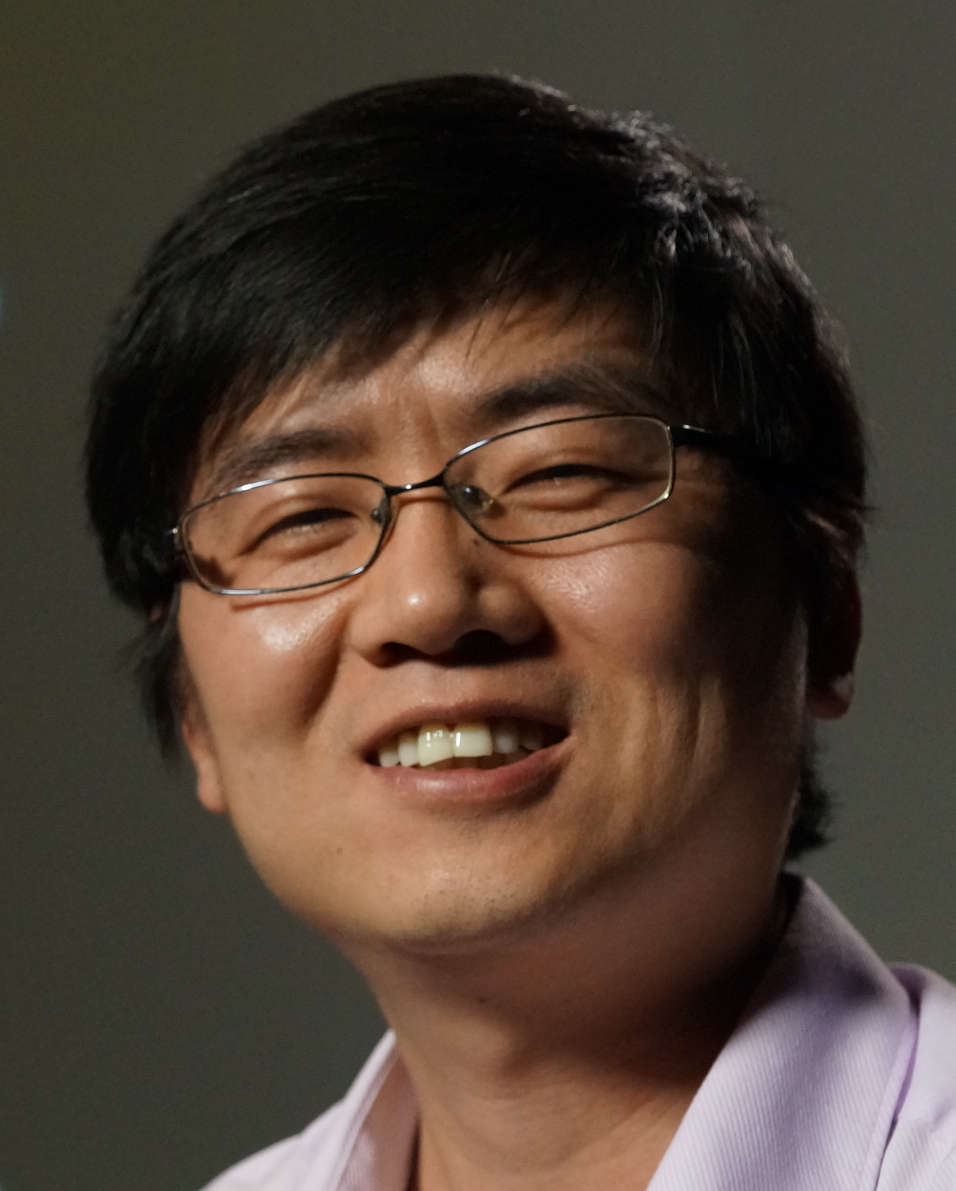
\includegraphics[width=1in,height=1.25in,clip,keepaspectratio]{hongbo}}]{Hongbu Fu}
is an Associate Professor in the School of Creative Media, City University of Hong Kong. He received the PhD degree in computer science from the Hong Kong University of Science and Technology in 2007 and the BS degree in information sciences from Peking University, China, in 2002. His primary research interests fall in the fields of computer graphics and human computer interaction. He has served as an associate editor of The Visual Computer, Computers \& Graphics, and Computer Graphics Forum.
\end{IEEEbiography}


\begin{IEEEbiography}[{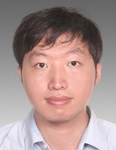
\includegraphics[width=1in,height=1.25in,clip,keepaspectratio]{sheng}}]{Bin Sheng}
received his BS degree in computer science from Huazhong University of Science and Technology in 2004, MS degree in software engineering from University of Macau in 2007, and PhD Degree in computer science from The Chinese University of Hong Kong in 2011. He is currently an associate professor in the Department of Computer Science and Engineering at Shanghai Jiao Tong University. His research interests include virtual reality, computer graphics, and image-based techniques.
\end{IEEEbiography}

\begin{IEEEbiography}[{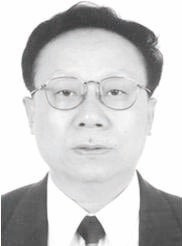
\includegraphics[width=1in,height=1.25in,clip,keepaspectratio]{wu}}]{Enhua Wu}
received the BS degree from Tsinghua University in 1970, and the PhD degree from the University of Manchester (UK) in 1984. He is currently a research professor at the Institute of Software, Chinese Academy of Sciences, and Fellow of China Computer Federation. He has also been teaching at the University of Macau since 1997, where he is currently an Emeritus Professor. His research interests include realistic image synthesis, virtual reality, and scientific visualization. He has served as an associate editor of The Visual Computer, Computer Animation and Virtual Worlds.
\end{IEEEbiography}




\end{document}


